% fichier Exposé-MontPellibre-juil2020/intro-programmation-sous-Linux.tex
\documentclass[xcolor=svgnames,final,smaller,a4]{beamer}
\usepackage{relsize}
\usepackage{luacode}
\usepackage{xcolor}
\usepackage{alltt}
\usepackage{wasysym}
\usepackage{verbatim}
\usepackage{hyperref}
\usepackage{newunicodechar}

% see also http://www.sascha-frank.com/Arrow/latex-arrows.html
% and http://tug.ctan.org/info/symbols/comprehensive/symbols-a4.pdf
% and https://ctan.math.illinois.edu/macros/latex/contrib/newunicodechar/newunicodechar.pdf
%%%% keep in order
%U+21A6 RIGHTWARDS ARROW FROM BAR
\newunicodechar{↦}{$\mapsto$}
%U+21B3 DOWNWARDS ARROW WITH TIP RIGHTWARDS
\newunicodechar{↳}{\rotatebox[origin=c]{180}{$\Lsh$}}
%U+2208 ELEMENT OF
\newunicodechar{∈}{$\in$}
% U+00AB LEFT-POINTING DOUBLE ANGLE QUOTATION MARK
\newunicodechar{«}{\guillemotleft}
% U+00BB RIGHT-POINTING DOUBLE ANGLE QUOTATION MARK
\newunicodechar{»}{\guillemotright}
% U+00B1 PLUS-MINUS SIGN
\newunicodechar{±}{$\pm$}
% U+00B5 MICRO SIGN
\newunicodechar{µ}{$\mu$}



\hypersetup{
  colorlinks   = true, %Colours links instead of ugly boxes
  urlcolor     = NavyBlue, %Colour for external hyperlinks
  linkcolor    = DarkGreen, %Colour of internal links
  citecolor   = DarkMagenta, %Colour of citations
  frenchlinks = true,
}

\usetheme{Montpellier}



\title{\textsc{Introduction à la Programmation} \\
(sous Linux)}
\author[B.Starynkevitch]{Basile \textsc{Starynkévitch} - \href{http://starynkevitch.net/Basile/}{\texttt{starynkevitch.net/Basile}}\\ \href{mailto:basile@starynkevitch.net}{\color{blue}{\texttt{basile@starynkevitch.net}}}
} %
\institute{MontPellibre (Montpellier)}
\date{été 2020}

\begin{document}
 \begin{luacode*}
   local gitpip=io.popen("git log --no-color --format=oneline -1 --abbrev=16 --abbrev-commit -q | cut -d' ' -f1")
   gitid=gitpip:read()
   gitpip:close()
 \end{luacode*}
  \newcommand{\mygitid}{\luadirect{tex.print(gitid)}}

%{% open a Local TeX Group
%\setbeamertemplate{sidebar}{}
 \begin{frame}
   
   
   \begin{relsize}{-1.5}
        \titlepage
        \textcolor{brown}{{\large \textbf{Les opinions me sont personnelles}} }
        
        \begin{center}
          git \texttt{\mygitid} ~ 
          \href{https://montpellibre.fr/spip.php?article4875}{https://montpellibre.fr/spip.php?article4875}

          Suivre les \href{https://fr.wikipedia.org/wiki/Hyperlien}{hyperliens} donnés ici.
        \end{center}
   \end{relsize}
\end{frame}
%}% end Local TeX Group

 \begin{frame}
    \frametitle{Licence}
    
    Ces transparents sont sous licence \href{https://creativecommons.org/licenses/by-sa/4.0/}{
\includegraphics[scale=0.75]{CC-BY-SA-4}} \relsize{-1}{(CC-BY-SA-4)}

    \vspace{1cm}
          Le code \LaTeX ~ (\texttt{lualatex}) de cette présentation est en \href{https://github.com/bstarynk/introprog-montpellibre-2020/}{\texttt{github.com/bstarynk/introprog-montpellibre-2020}}
 \end{frame}
 
 \begin{frame}
    \frametitle{Plan}
    
   \tableofcontents
 \end{frame}


 \AtBeginSection[]{
   \begin{frame}{Sommaire}
     \small \tableofcontents[currentsection, hideothersubsections]
   \end{frame}
 }


 %%++++++++++++++++++++++++++++++++++++++++++++++++++++++++++++++++++++++
\section{Introduction}

\begin{frame}
  \frametitle{Introduction}
  \framesubtitle{les puissances, les bases, les nombres, les logarithmes}

  Les \textbf{puissances de dix}: $10^1 = 10$, $10^2 = 10 \times 10 = 100$,
  $10^3 = 10 \times 10 \times 10 = 1000$, etc.... Par convention $10^0 = 1$. \\
  Réciproque: \textbf{logarithme décimal}: $log_{10} 1000 = 3$ (car $10^3 = 10000$)

  \vspace{0.5cm}
  
  Les  \textbf{puissances de deux}: $2^1 = 2$, $2^2 = 2 \times 2 = 4$, $2^3 = 2 \times 2 \times 2 = 8$, $2^4 = 2 \times 2 \times 2  \times 2 = 16$, etc.... Par convention $2^0 = 1$. \\ Réciproque: \textbf{logarithme binaire}: $log_2 16 = 4$ (car $16 = 2^4$) et $log_2 4 = 2$

  \vspace{0.5cm}

  Notation décimale (base dix) et binaire (base deux) des nombres entiers: \\
  \emph{cent vingt trois}, c'est \textbf{en base dix}, $123 = 1 \times 10^2 + 2 \times 10^1 + 3 \times 10^0$ \\
  \emph{douze}, c'est \textbf{en base deux}, $1100 = 1 \times 2^3 + 1 \times 2^2 + 0 \times 2^1 + 0 \times 2^0$
\end{frame}


\begin{frame}
  \frametitle{Introduction}
  \framesubtitle{Qu'est ce que l'information}

  \begin{block}{un bit}

    \textbf{Quantité ``élémentaire'' d'information}. \textcolor{red}{Le jeu de pile ou face} transmet approximativement \textcolor{purple}{\textbf{un bit}}, car il y a $2 = 2^1$ possibilités
    
  \end{block}

  Remarques:
  \begin{itemize}
  \item on a fait \textbf{abstraction} des autres possibilités (la pièce perdue dans le caniveau ...)
  \item on a fait une \textbf{simplification} et une \textbf{modélisation} de la réalité.
    \item on a évidemment $log_2 ~ 2 = 1$ car $2 = 2^1$
  \end{itemize}

  Mais l'\emph{abstraction}, la \emph{simplification}, la \emph{modélisation} sont \textbf{au c{\oe}ur de l'activité de programmation}.
  
\end{frame}

\begin{frame}
  \frametitle{Introduction}
  \framesubtitle{Combien de bits transmis au jeu de dés?}
  
  \textbf{un dé a 6 faces}, donc plus de 2 et moins de 3 bits transmis, puisque
  $4 = 2^2 < 6 < 2^3 = 8$

  \vspace{1cm}

  \emph{``informatiquement''} on a transmis $log_2~ 6$ bits, donc $\approx 2,58496$ bits

  \vspace{1cm}

  Q: \textit{combien de bits (environ) pour le jeu de la roulette?} (36 cas)
  
\end{frame}

\begin{frame}
  \frametitle{Introduction}
  \framesubtitle{Que faire avec un bit}

  
  \textbf{Représenter toutes choses à deux possibilités}
  
  \begin{itemize}

  \item valeur de vérité en logique : \textbf{vrai} ou \textbf{faux}

  \item comparaison ($<$ ou $>$) entre deux grandeurs (longueur, tension électrique, etc...)
  \item chiffre binaire

    \item signe $+$ ou $-$
  \end{itemize}

  \vspace{1cm}

  \textbf{Distinction entre \textcolor{red}{chiffre} et \textcolor{red}{nombre}}
\end{frame}

\begin{frame}
  \frametitle{Introduction}
  \framesubtitle{Comment représenter \emph{physiquement} un bit}

  Utiliser, ou simplifier, par un \textbf{phénomène physique à \textcolor{red}{deux états}}

  \begin{itemize}
  \item interrupteur marche/arrêt (donc tension électrique: $\approx 0V$ vs $1V$ à $3V$)
  \item pendule mécanique (à gauche ou à droite), horlogerie (Babbage)
    \item onde sonore
    \item magnétisation (tambour, disque dur)
  \item tubes à vide (ENIAC), transistors, circuits intégrés
  \item etc...
  \end{itemize}
  
  \vspace{2mm}
 
  NB. Certaines technologies {\relsize{-1}{(mémoire Flash, SSD, Clefs USB)}} représentent deux bits par 4 états. 
  Mais le matériel est imparfait.
\end{frame}


\begin{frame}
  \frametitle{Introduction}
  \framesubtitle{Notation décimale, binaire,  octale, hexadécimale des nombres entiers}


  \begin{itemize}
    \item
    \textit
   {cent vingt trois} = $123$ \textcolor{red}{en décimal}
  car $1 \times 10^2 + 2 \times 10^1 + 3 \times 10^0$

  \item
  \textit{dix} = $1010_b$ ou \texttt{0b1010}
  \textcolor{red}{en binaire} (binary digit = bit)
  car $1  \times 2^3 + 0 \times 2^2 + 1 \times 2^1 + 0 \times 2^0$

  \item
  \textit{douze} = $14_o$ ou \texttt{014} ou \texttt{0o14}
  \textcolor{red}{en octal}
  car $1  \times 8^1 + 4 \times 8^0$

  \item \textit{vingt} =  $14_h$ ou \texttt{0x14}
  \textcolor{red}{en hexadécimal}
  car $1  \times 16^1 + 4 \times 16^0$. Les chiffres après 9 sont A ($=10$), B, C, D, E, F ($=15$). \\
  Donc \texttt{0x1a} est vingt-six.
 
  \end{itemize}
  
  \vspace{1cm}
  Remarque: un chiffre octal correspond à 3 bits (par exemple $5_o = 101_2$); un chiffre hexadécimal correspond à 4 bits (par exemple $11 = B = 1011_2$).
\end{frame}
\begin{frame}
  \frametitle{Introduction}
  \framesubtitle{Octets}

Un  \textcolor{red}{\textbf{octet}} (anglais: \textit{byte}) contient huit bits.

\begin{itemize}
\item petit entier entre $0$ et $2^8-1$ donc $255$

\item entier signé entre -128 ($-2^7$) et +127 ($2^7-1$)

\item codage de caractères (lettres, chiffres, ponctuation)
  \href{https://en.wikipedia.org/wiki/ASCII}{en.wikipedia.org/wiki/ASCII}\\
  \textcolor{brown}{\texttt{A}} codé 65,  \textcolor{brown}{\texttt{C}} codé 67,  \textcolor{brown}{\texttt{Z}} codé 90,   \textcolor{brown}{\texttt{a}} codé 97,  \textcolor{brown}{\texttt{?}} codé 63

\item codage universel Unicode UTF-8 sur un à quatre octets
\href{https://en.wikipedia.org/wiki/UTF-8}{\texttt{en.wikipedia.org/wiki/UTF-8}}
et \href{https://utf8everywhere.org/}{\texttt{utf8everywhere.org}}. \\ Par exemple \textcolor{brown}{\texttt{°}} codé sur deux octets \texttt{0xc2} \texttt{0xb0}

\end{itemize}
\end{frame}



\begin{frame}
  \frametitle{Introduction}
  \framesubtitle{Circuits logiques combinatoires}

Voir \href{https://www.positron-libre.com/cours/electronique/logique-combinatoire/}{\texttt{www.positron-libre.com/cours/electronique/logique-combinatoire/}}

\vspace{0.5cm}

 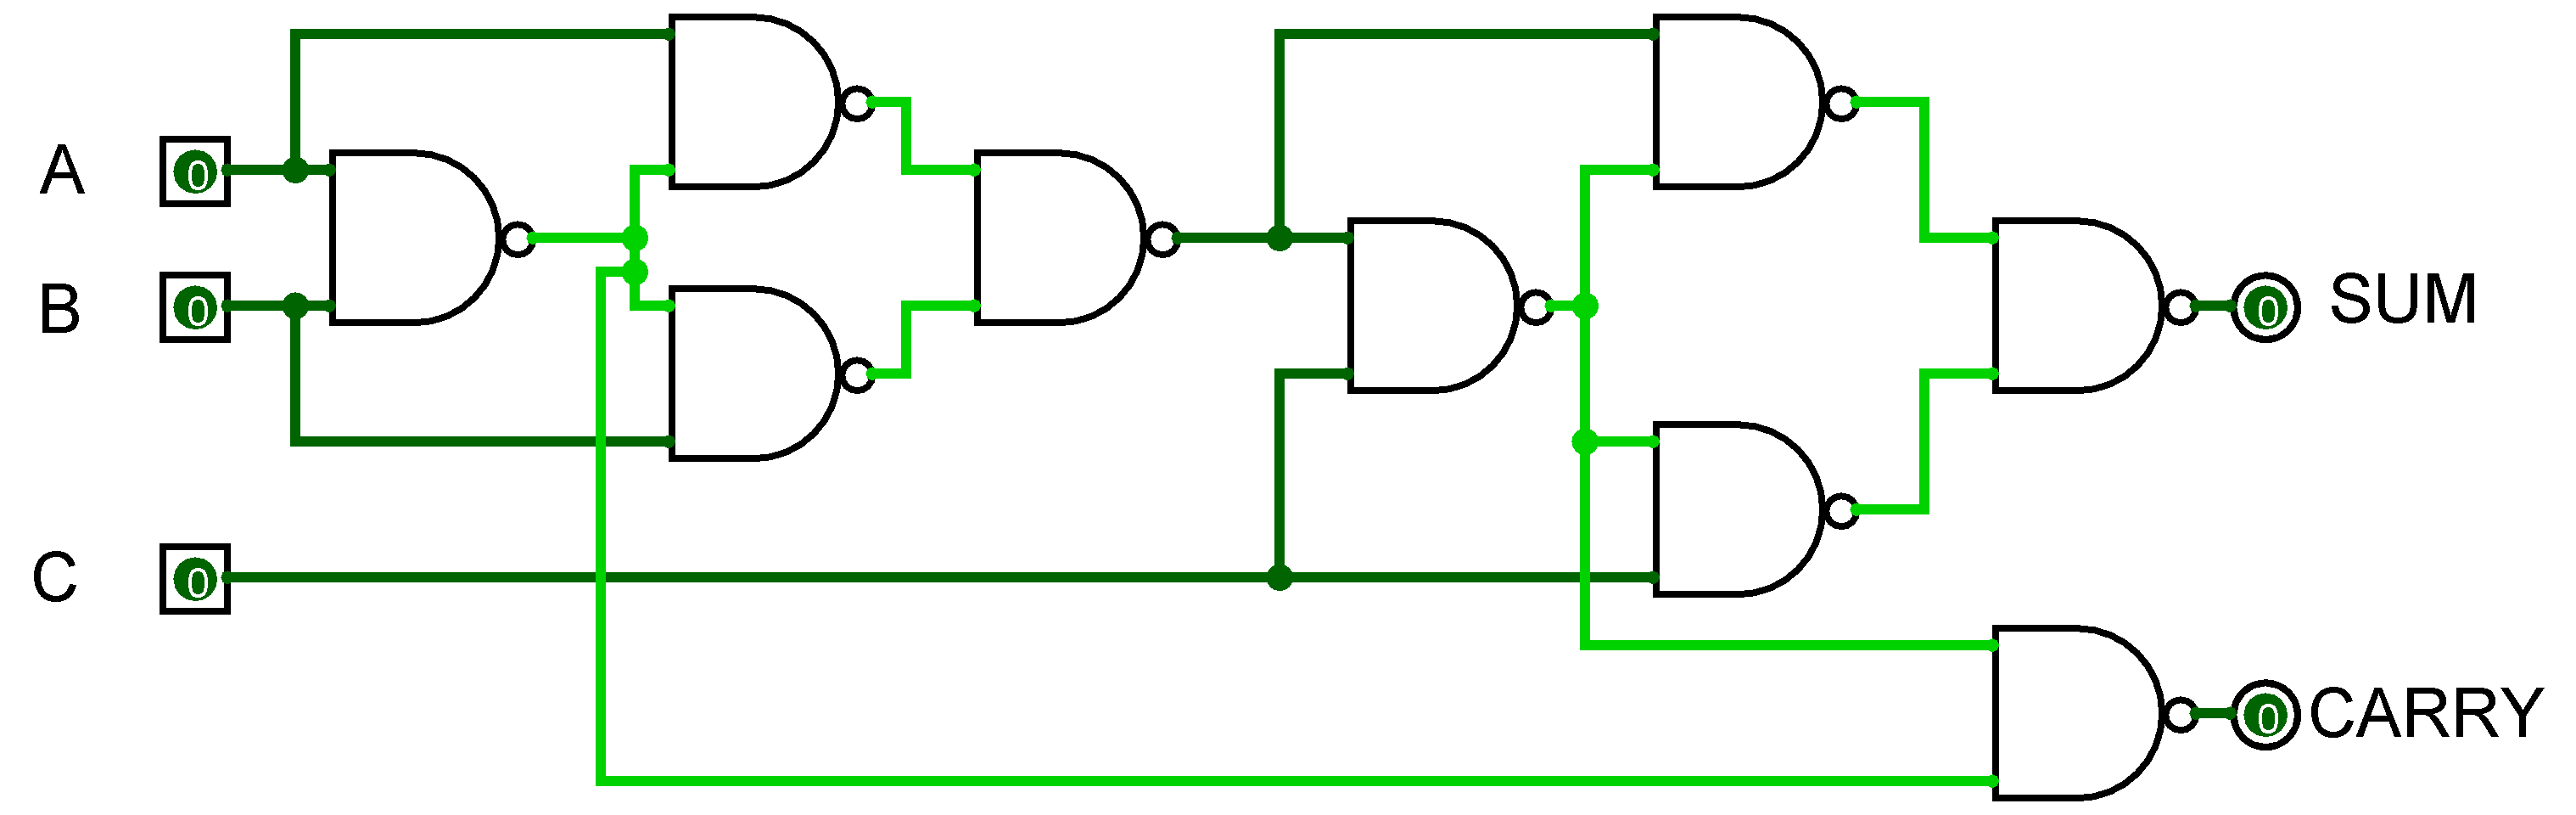
\includegraphics[width=0.7\textwidth]{Full-Adder-Nand}

 \vspace{0.5cm}

 Additionneur un bit avec retenue à base de portes \textbf{NAND} (et-non)
 
Les portes \textbf{NAND} ou \textbf{NOR} sont \textit{universelles} et simples à réaliser (quelques transistors).


\end{frame}


\begin{frame}
  \frametitle{Introduction}
  \framesubtitle{Circuits logiques circulaires}

La bascule flip-flop (verrou RS) à deux portes  \textbf{NOR} (ou-non) têtes-bêches mémorise un bit.

\vspace{0.5cm}


 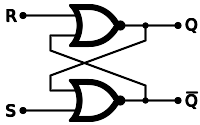
\includegraphics[width=0.6\textwidth]{RS-Flip-flop}



\vspace{0.5cm}

Voir \href{http://www.paturage.be/electro/inforauto/portes/bascule.html}{www.paturage.be/electro/inforauto/portes/bascule.html}

\end{frame}



\begin{frame}
  \frametitle{Introduction}
  \framesubtitle{Combinaisons de portes logiques}

En combinant beaucoup (millions) de portes logiques on produit les microprocesseurs actuels (milliard de transistors, 
AMD ThreadRipper Ryzen)

\vspace{0.5cm}

 \href{https://cdn.arstechnica.net/wp-content/uploads/2017/02/ryzen-die.jpg}{\texttt{cdn.arstechnica.net/wp-content/uploads/2017/02/ryzen-die.jpg}}

 \vspace{0.5cm}
 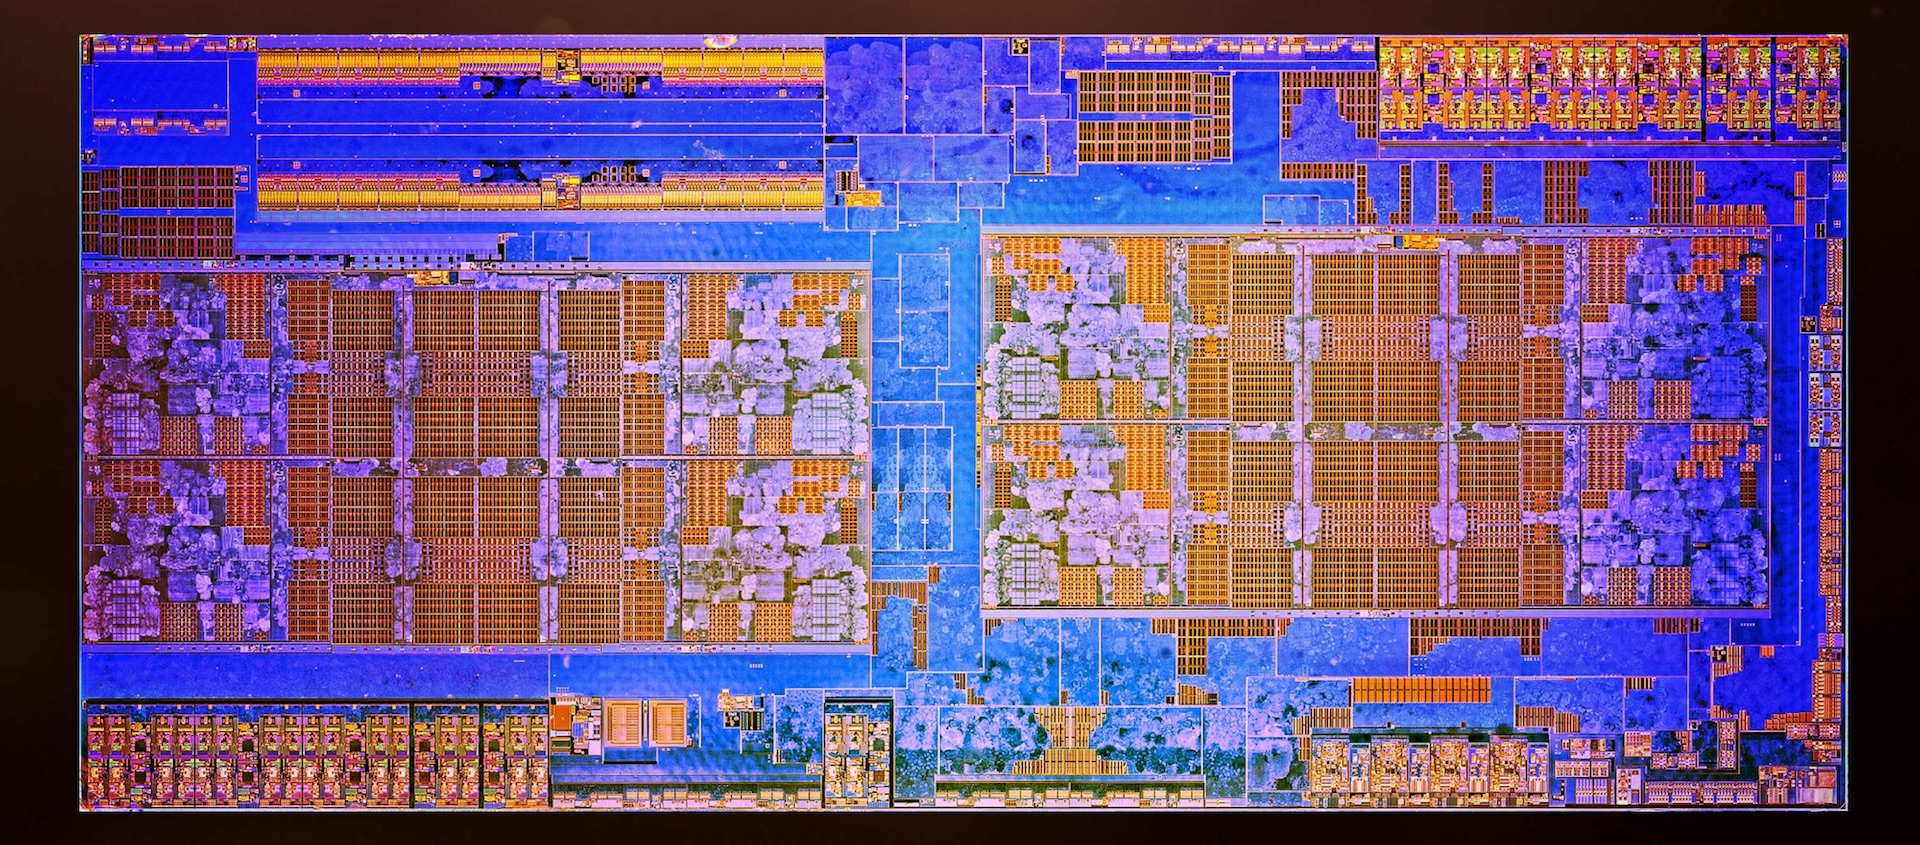
\includegraphics[width=0.7\textwidth]{ryzen-die.jpg}

\end{frame}

\begin{frame}
  \frametitle{Introduction}
  \framesubtitle{Ordres de grandeurs économiques en 2020}

\begin{itemize}
\item investissement pour la R\&D, la fabrication, l'usine pour un microprocesseur haut de gamme: dix milliards de US\$
\item nombre de transistors par puce: milliard (sur quelques centimètres carrés)
\item prix de vente (après test): environ mille dollars / pièce (milliers)
\item taux de rendement: quelques pourcents, la plupart des puces sont défaillantes
\item taux de panne par porte : moins d'une défaillance par heure
\item consommation énergetique du numérique: quelques pourcents de la production électrique française
\item prix de vente d'un ordinateur: centaines d'euros.
\item plusieurs "ordinateurs" par habitant (microcontrôleurs, informatique embarquée, téléphones portables, datacenters)
  \item productivité d'un développeur: quelques dizaines de milliers de ligne de code source par an.
\end{itemize}
\end{frame}

\begin{frame}
  \frametitle{Introduction}
  \framesubtitle{Ordres de grandeurs technologiques en 2020}
 
\begin{itemize}
\item 8 c{\oe}urs de processeur à 3GHz
\item mémoire cache: 16 Mo (accès 10ns, bande passante 0,5To/s)
\item taille mémoire RAM d'un ordinateur : 32 Goctets
\item temps d'accès RAM: 200 ns
\item bande passante RAM: centaine Mo/seconde
\item taille disque SSD : un demi téra-octet
\item puissance thermique dissipée en charge: 250W
\item temps d'accès SSD: 50 microsecondes pour un bloc de 4Ko.
\end{itemize}

\end{frame}

\begin{frame}

  \frametitle{Introduction}
  \framesubtitle{Vue interne d'un ordinateur de bureau en 2020}

\href{https://images.app.goo.gl/BMQxP7c4Zcyrh3XD7}{images.app.goo.gl/BMQxP7c4Zcyrh3XD7}

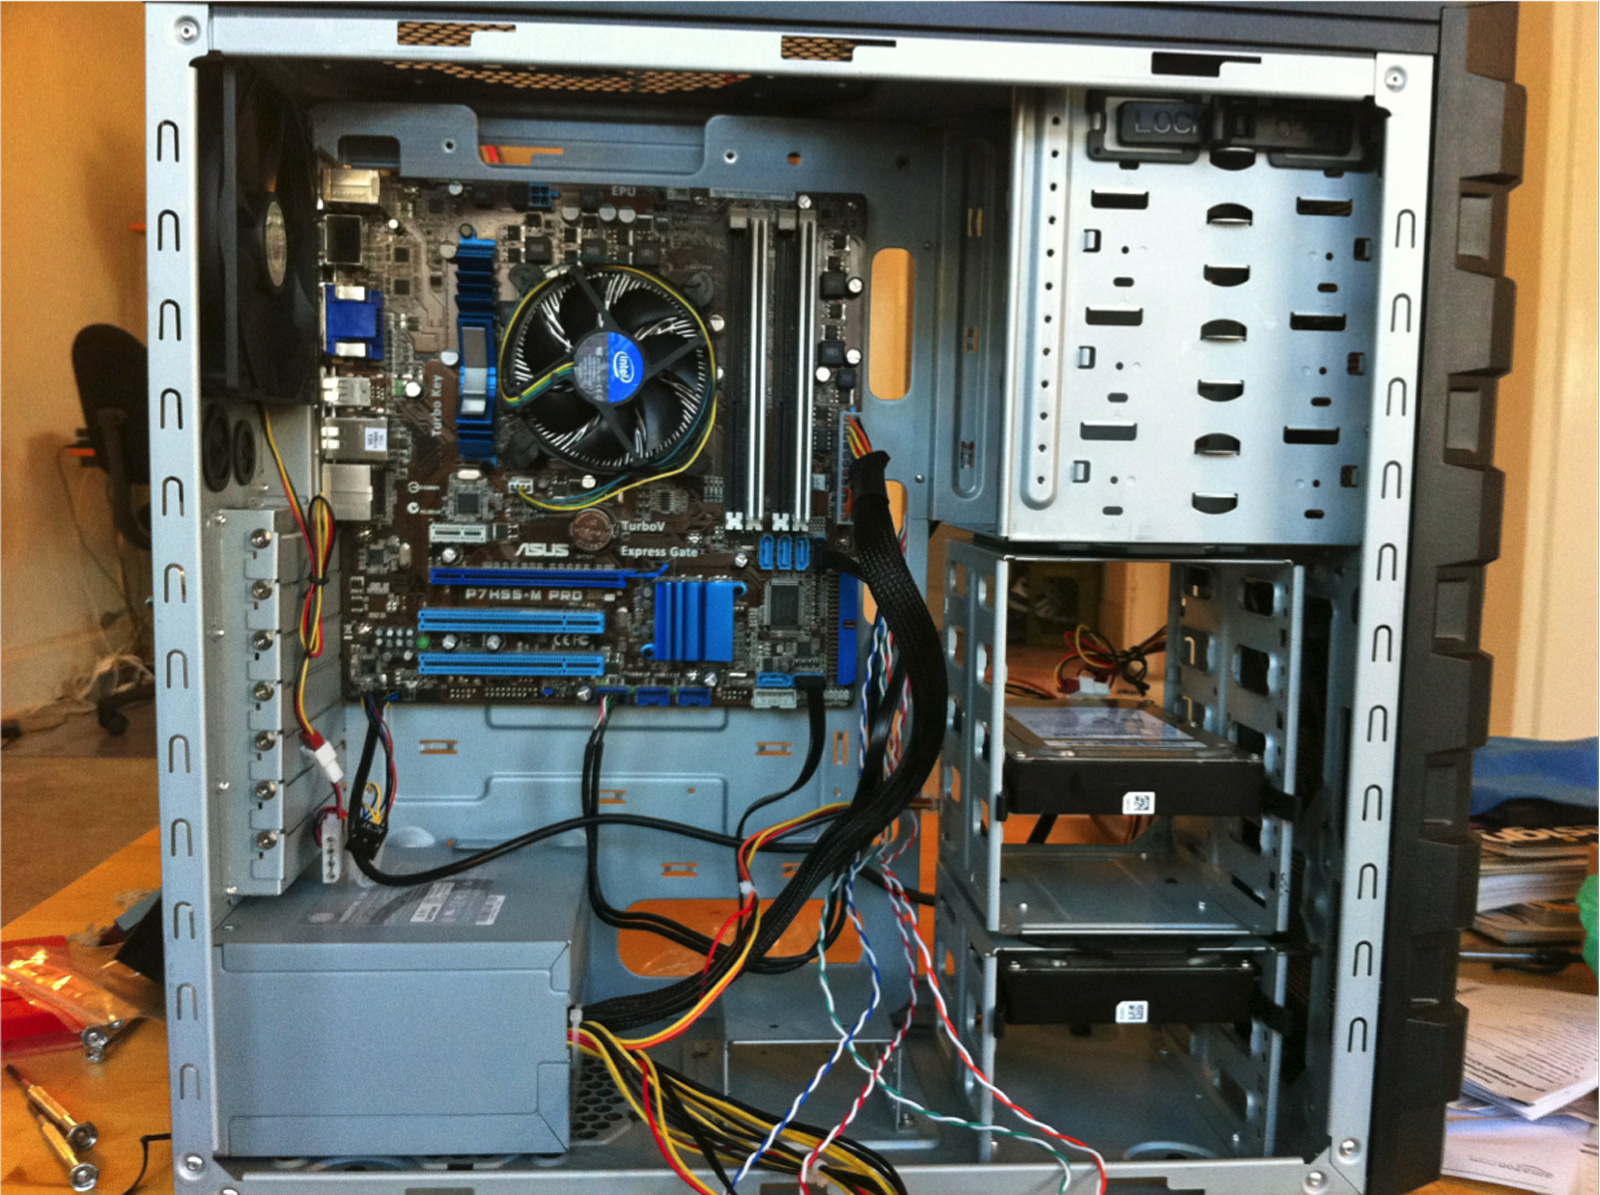
\includegraphics[width=0.66\textwidth]{interieur-ordinateur.png}
\end{frame}


 %%++++++++++++++++++++++++++++++++++++++++++++++++++++++++++++++++++++++
\section{couches logicielles}

%%%%%%%%%%%%%%%%%%%%%%%%%%%%%%%%%%%%%%%%%%%%%%%%%%%%%%%%%%%%%%%%
\subsection{généralités sur le logiciel}

\begin{frame}
  \frametitle{Couches logicielles}
  \framesubtitle{Les différents types de logiciels}

\begin{itemize}

\item logiciel et langage de description des circuits (VHDL, SystemC)
\item firmware - interne à la souris (langage machine 8051), au disque dur, à la carte réseau
\item logiciel de démarrage (UEFI, BIOS): charge le système d'exploitation
\item noyau (par exemple Linux) du système d'exploitation, gère les fichiers et les processus
\item utilitaires systèmes (gestion du réseau, ...)
\item interface graphique ou navigateur Web
\item bibliothèques logicielles standard (\href{http://qt.io}{Qt}, \texttt{libc})
\item outils logiciels pour le développeur (compilateur)
\item logiciels applicatifs (bureautique) ou métiers (aéronautique)
\item scripts utilisateurs et fichiers de configuration
\item commandes, schémas de bases de données, langage d'imprimante (PDF, ...)

\end{itemize}
\end{frame}

\begin{frame}
  \frametitle{Couches logicielles}
  \framesubtitle{Aspects légaux (code pénal)}

  En France

  
  \begin{block}{article 323-1 et suivants du Code Pénal}

    \begin{relsize}{-0.5}
Le fait d'accéder ou de se maintenir, frauduleusement, dans tout ou
partie d'un système de traitement automatisé de données est puni de
deux ans d'emprisonnement et de 60 000 € d'amende.

Lorsqu'il en est résulté soit la suppression ou la modification de
données contenues dans le système, soit une altération du
fonctionnement de ce système, la peine est de trois ans
d'emprisonnement et de 100 000 € d'amende.

Lorsque les infractions prévues aux deux premiers alinéas ont été
commises à l'encontre d'un système de traitement automatisé de données
à caractère personnel mis en œuvre par l'Etat, la peine est portée à
cinq ans d'emprisonnement et à 150 000 € d'amende.
    \end{relsize}
  \end{block}
\end{frame}



\begin{frame}
  \frametitle{Couches logicielles}
  \framesubtitle{Aspects légaux (RGPD)}

  En Europe, obligation d'avoir le consentement éclairé et préalable
  pour tout traitement de données à caractère
  personnel. \textbf{\textcolor{red}{Règlement Général sur la
      Protection des Données}}

 \vspace{0.5cm}
  Voir
  \href{https://donnees-rgpd.fr/definitions/rgpd-pour-les-nuls/}{\texttt{donnees-rgpd.fr/definitions/rgpd-pour-les-nuls}}, \href{https://www.laquadrature.net}{\texttt{www.laquadrature.net}} et \href{https://april.org/}{\texttt{april.org}} 
  pour en savoir plus.
  
  \vspace{0.5cm}

  \textcolor{red}{Les pénalités sont dissuasives}
\end{frame}

\begin{frame}
  \frametitle{Couches logicielles}
  \framesubtitle{Aspects légaux (copyright et logiciels libres, brevets logiciels, vente liée)}

  \textbf{copyrights logiciels et logiciels libres:} Voir
  \href{https://april.org/}{\texttt{april.org}} et
  \href{https://aful.org/}{\texttt{aful.org}} et
  \href{https://www.eff.org/}{\texttt{eff.org}} et
  \href{https://www.fsf.org/}{\texttt{fsf.org}} et
  \href{https://opensource.org/}{\texttt{opensource.org}} et
   \href{https://adullact.org/}{\texttt{adullact.org}} et
  \href{https://montpellibre.fr/}{\texttt{montpellibre.fr}} et
   \href{https://cecill.info/}{\texttt{cecill.info}} \textcolor{red}{\textit{etc...}}
  (ou votre juriste préféré)
    pour en savoir
    plus.

    \vspace{0.5cm}
    \textbf{Vente liée matériel + logiciel :} voir
    \href{https://non.aux.racketiciels.info/}{\texttt{non.aux.racketiciels.info}}
    et
    \href{https://bons-constructeurs-ordinateurs.info/}{\texttt{bons-constructeurs-ordinateurs.info}}
    
    \vspace{0.5cm}

    NB. \textbf{Ne pas inventer sa propre licence logicielle libre} sans
    assistance juridique: le droit est aussi complexe que
    l'informatique!
   
    \vspace{0.3cm}
 
    PS. Attention aux incompatibilités de licences logicielles entre composants logiciels
\end{frame}


\begin{frame}
  \frametitle{Couches logicielles}
  \framesubtitle{Aspects techniques et sociaux}

  \textbf{Code binaire} ou \textbf{code machine} \\
  Il est executé par l'ordinateur. Totalement illisible.
  \textcolor{red}{\textbf{Toujours généré}} par d'autres logiciels.

    \vspace{0.3cm}
  \textbf{Code source} \\
  \textcolor{red}{Il est écrit par l'informaticien et partagé avec d'autres développeurs}.
  Contient plein de choses pour les humains, inutiles aux ordinateurs.

    \vspace{0.3cm}
  \textbf{Code intermédiaire} \\
  Des logiciels transforment le code source en code binaire, en passant par des representations intermédiaires. Dont le  \textbf{code objet} (``object code'') et les bibliothèques partagées (``shared libraries'').
  
    \vspace{0.3cm}
    \textbf{Méta-programmation} \\
    Beaucoup de logiciels manipulent, analysent, générent, gérent du code. Méta-programmer, c'est écrire \textcolor{red}{un programme qui manipule le code d'autres programmes}.
\end{frame}


%%%%%%%%%%%%%%%%%%%%%%%%%%%%%%%%%%%%%%%%%%%%%%%%%%%%%%%%%%%%%%%%
\subsection{architecture des microprocesseurs}
\begin{frame}
  \frametitle{logiciel et architecture des microprocesseurs}
  \framesubtitle{Jeu d'instructions machine, registres, conventions d'appel}

  \textcolor{DarkGreen}{application binary interface}. Document (parfois, 800 pages)
  décrivant le comportement souhaité d'un microprocesseur et son
  \textbf{jeu d'instructions machine} (``instruction set architecture'')

    \vspace{0.3cm}
  \textcolor{red}{\textbf{registres d'un processeur}}. Mémoire
  ultra-rapide sur la puce. Souvent, une à trois douzaines de mots de
 16, 32 ou 64 bits
    \vspace{0.3cm}
    
    \textcolor{red}{\textbf{conventions d'appel}}. Règles d'usage des registres, pour des sous-programmes différents puissent être assemblés ensemble.


    \vspace{0.3cm}
    \textcolor{red}{\textbf{exemples}}: {\large \href{https://riscv.org/}{\texttt{riscv.org}}} (cartes graphiques, microcontroleurs), \href{https://en.wikipedia.org/wiki/X86-64/}{\texttt{x86-64}} (PCs actuels), \href{https://fr.wikipedia.org/wiki/Architecture_ARM}{ARM} (tablettes, téléphones, automobile), \textsc{PowerPC}
    \vspace{0.3cm}
    
    Le x86 (tous nos PCs) est \emph{très complexe} pour des raisons
    historiques de compatibilité ascendante. Une vue pédagogique
    simplifiée est le \href{http://siever.info/cs400/Y86.html}{Y86}
    (fictif).
\end{frame}

\begin{frame}
  \frametitle{logiciel et architecture des microprocesseurs}
  \framesubtitle{Exemple: PowerPC NXP 601 : broches et signaux}

  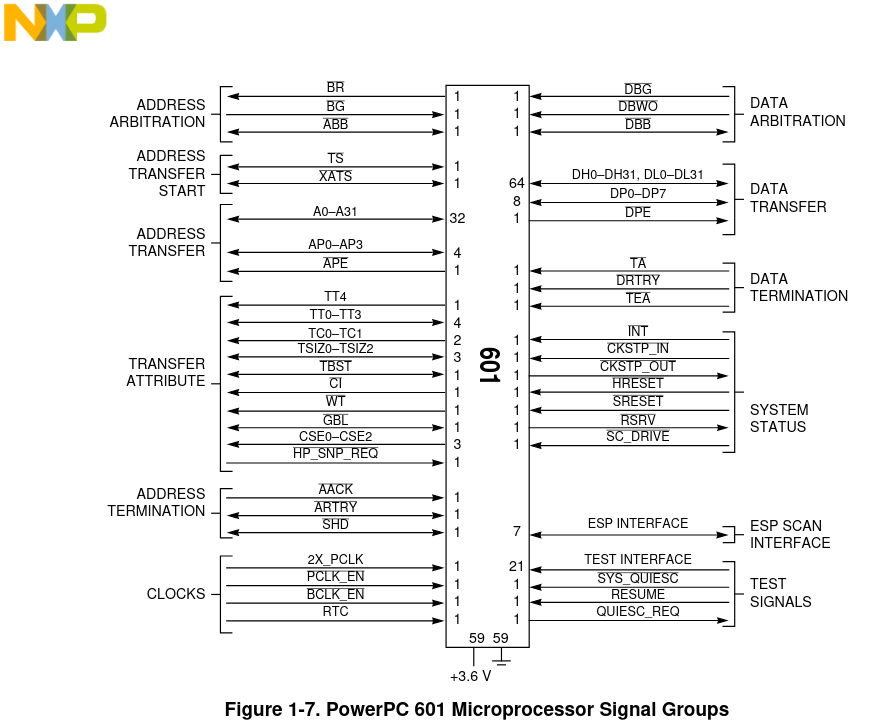
\includegraphics[width=0.85\textwidth]{powerpc-nxp-601}


\end{frame}
\begin{frame}
  \frametitle{logiciel et architecture des microprocesseurs}
  \framesubtitle{Exemple: PowerPC NXP 601 : microarchitecture}

  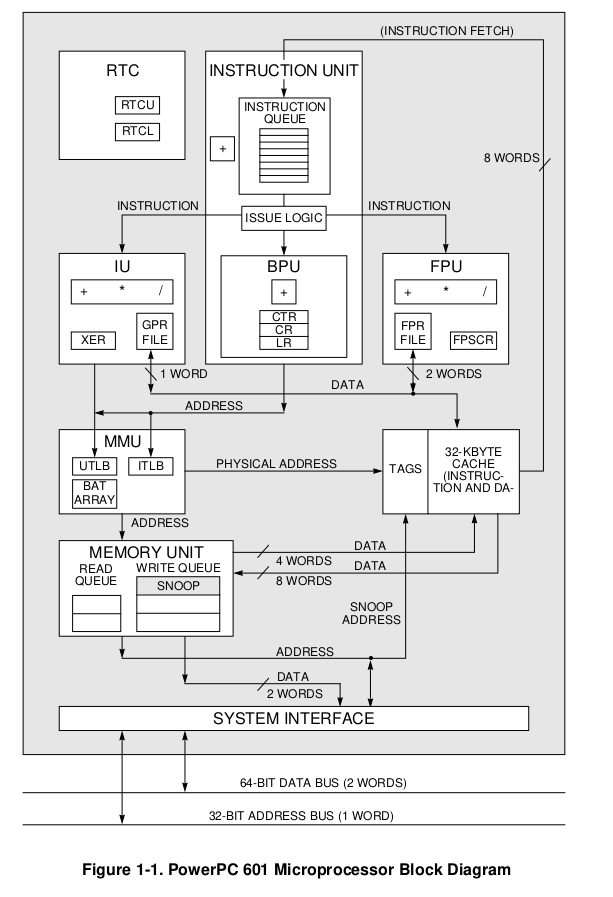
\includegraphics[width=0.50\textwidth]{powerpc601-microarchitecture}


\end{frame}

\begin{frame}
  \frametitle{logiciel et architecture des microprocesseurs}
  \framesubtitle{Exemple: Architecture PowerPC601 : registres complets}
  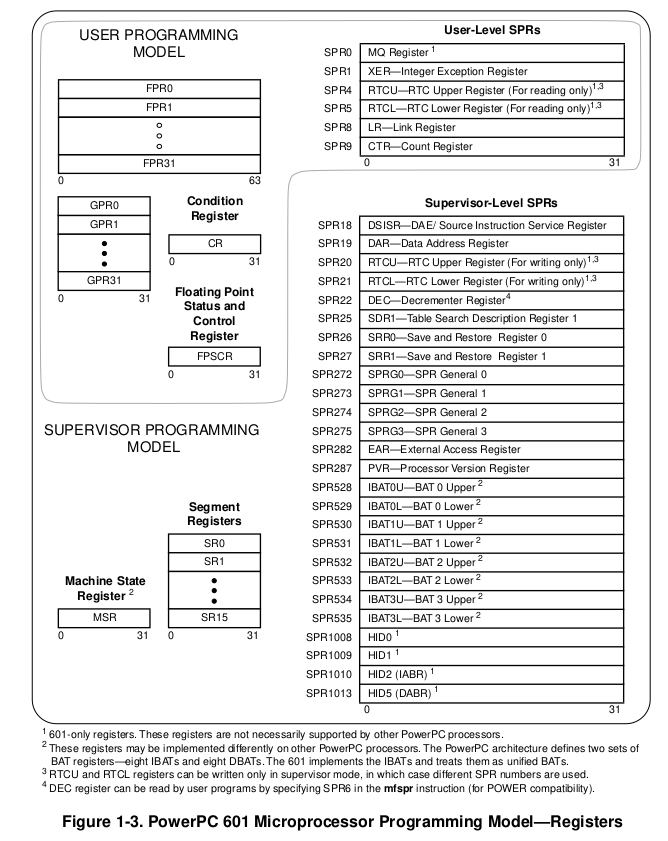
\includegraphics[width=0.6\textwidth]{powerpc-registers}
\end{frame}

\begin{frame}
  \frametitle{logiciel et architecture des microprocesseurs}
  \framesubtitle{Exemple: Architecture PowerPC : registres utilisateurs}

  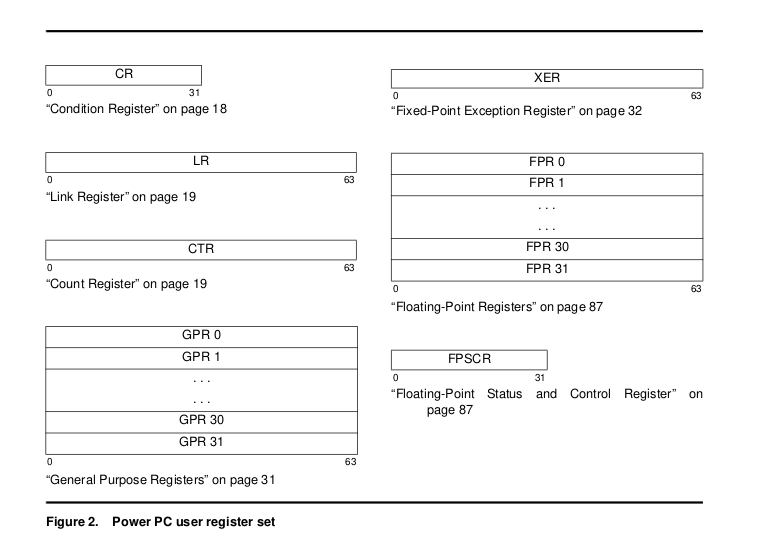
\includegraphics[width=0.85\textwidth]{powerpc-user-register}


  avec \texttt{GPR0} toujours à 0
\end{frame}

\begin{frame}
  \frametitle{logiciel et architecture des microprocesseurs}
  \framesubtitle{Exemple: Architecture x86-64 : registres utilisateurs}

  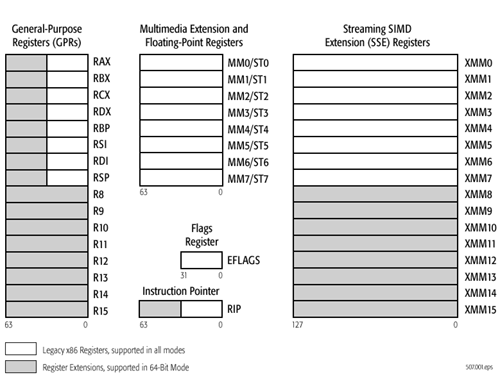
\includegraphics[width=0.75\textwidth]{x86-64-registers}


  où \texttt{RSP} est le pointeur de pile (``stack pointer'')
\end{frame}

\begin{frame}
  \frametitle{logiciel et architecture des microprocesseurs}
  \framesubtitle{Exemple: Architecture PowerPC : registre de conditions}

  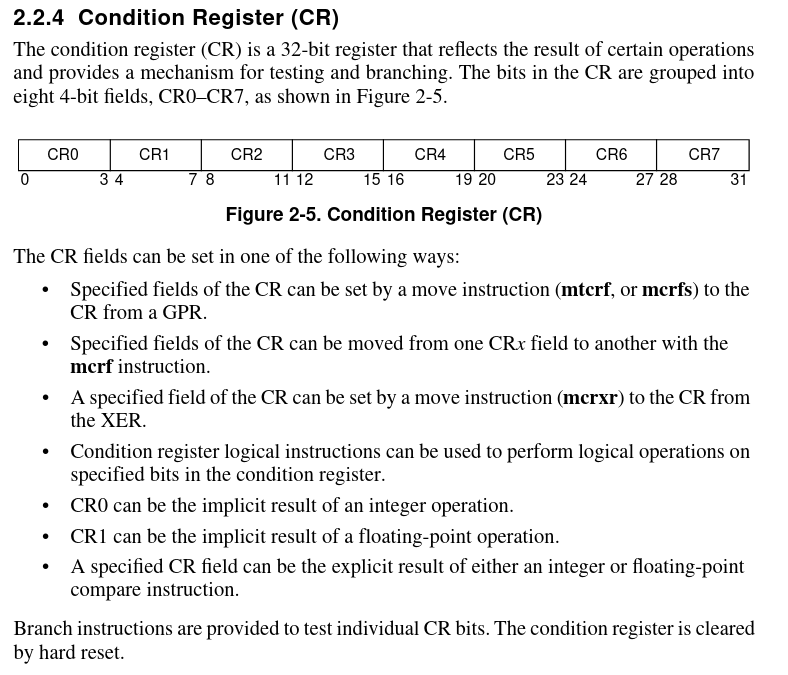
\includegraphics[width=0.75\textwidth]{powerpc-condreg}


\end{frame}

\begin{frame}
  \frametitle{logiciel et architecture des microprocesseurs}
  \framesubtitle{Exemple: Architecture PowerPC : registre d'état machine (MSR)}
  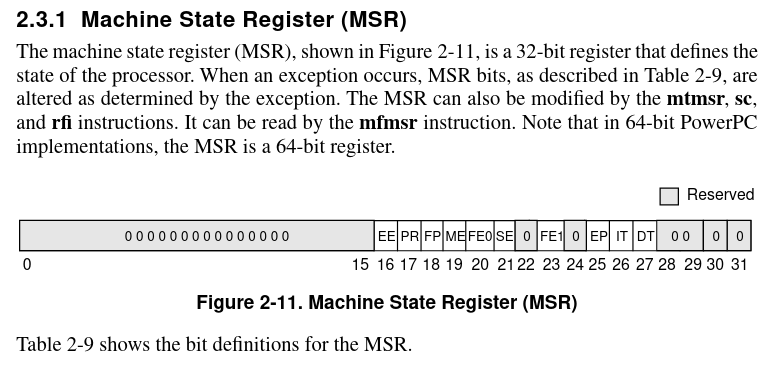
\includegraphics[width=0.75\textwidth]{powerpc-machstatereg}


  \vspace{0.3cm}

  Voir \href{https://www.nxp.com/files-static/32bit/doc/user_guide/MPC601UM.pdf}{\texttt{www.nxp.com/files-static/32bit/doc/user\_guide/MPC601UM.pdf}}
\end{frame}

\begin{frame}
  \frametitle{logiciel et architecture des microprocesseurs}
  \framesubtitle{Exemple: Architecture PowerPC : rôles des bits du registre d'état machine (MSR)}
  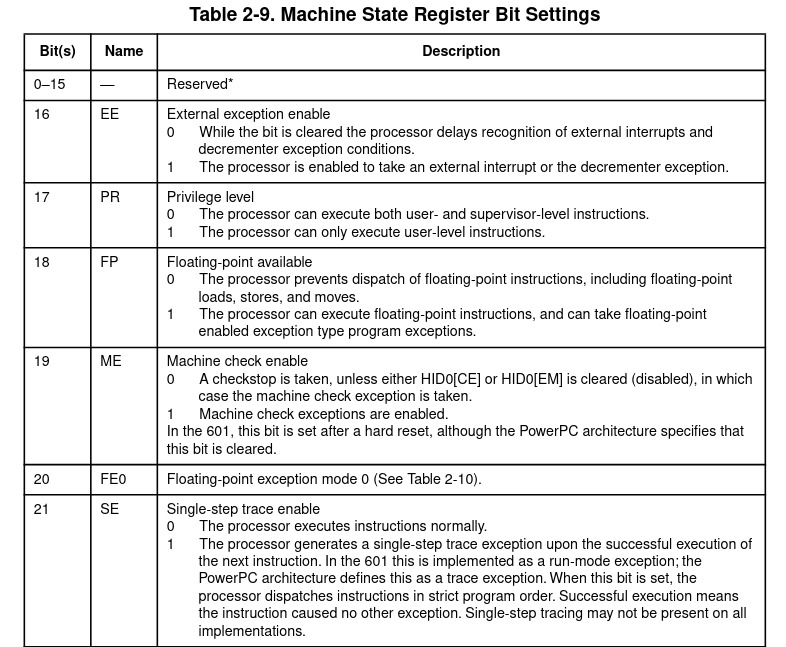
\includegraphics[width=0.75\textwidth]{powerpc-msr-bits}


\end{frame}

\begin{frame}
  \frametitle{logiciel et architecture des microprocesseurs}
  \framesubtitle{Deux modes de fonctionnement des microprocesseurs}

  \begin{itemize}
  \item \textcolor{red}{\textbf{mode superviseur}}: toutes les
    instructions machines sont permises, y compris les plus
    dangereuses (entrée/sorties physiques, configuration de l'espace
    d'addressage, modification de la fréquence ou de l'énergie
    consommée). Pour \textbf{le code du noyau} supposé  \textcolor{red}{\textbf{fiable et correct}}.

    \item \textcolor{red}{\textbf{mode utilisateur}}: les instructions
      machines dangereuses (E/S, mémoire virtuelle, ....)  sont
      interdites et ne sont pas executées. Pour \textbf{le code
        applicatif} : quand il plante, le système (noyau) prend la
      main.
    
  \end{itemize}


  Les \textcolor{red}{\textbf{interruptions}} font passer du mode
  utilisateur au mode superviseur. Elles sont \textbf{internes}
  {\relsize{-1}{(instruction illicite en mode utilisateur, division
      par 0, défaut de page, appel système...)}} ou \textbf{externes}
  {\relsize{-1}{(temporisation, surchauffe, paquet Ethernet reçu, fin de lecture
      d'un bloc du disque, ...)}}
\end{frame}

\begin{frame}
  \frametitle{logiciel et architecture des microprocesseurs}
  \framesubtitle{Exemple: Architecture PowerPC : formats d'instructions machine}
  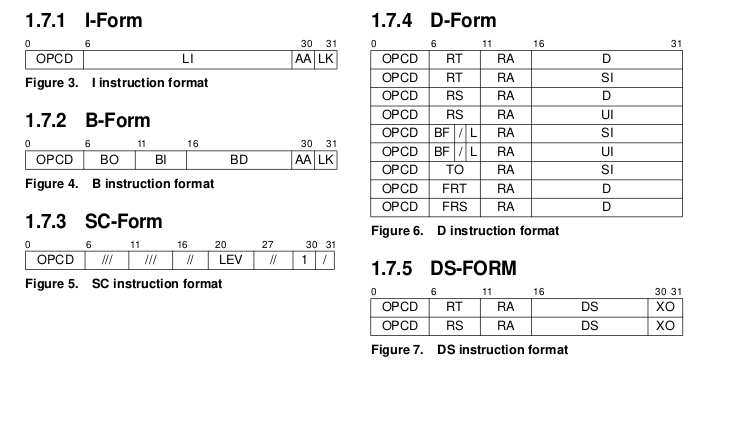
\includegraphics[width=0.9\textwidth]{powerpc-instr-format}
  

\end{frame}


\begin{frame}
  \frametitle{logiciel et architecture des microprocesseurs}
  \framesubtitle{Exemple: Architecture PowerPC : appel système}
  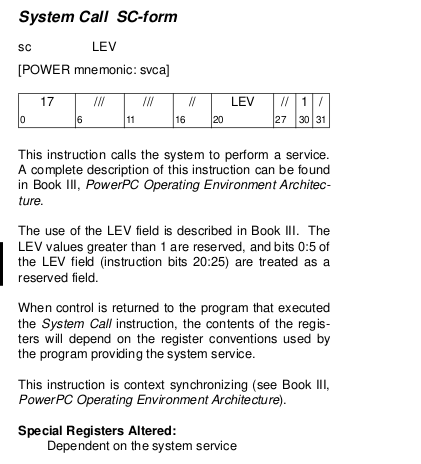
\includegraphics[width=0.60\textwidth]{powerpc-syscall-instr}
\end{frame}

\begin{frame}
  \frametitle{logiciel et architecture des microprocesseurs}
  \framesubtitle{Exemple: Architecture PowerPC : chargement d'un registre}
  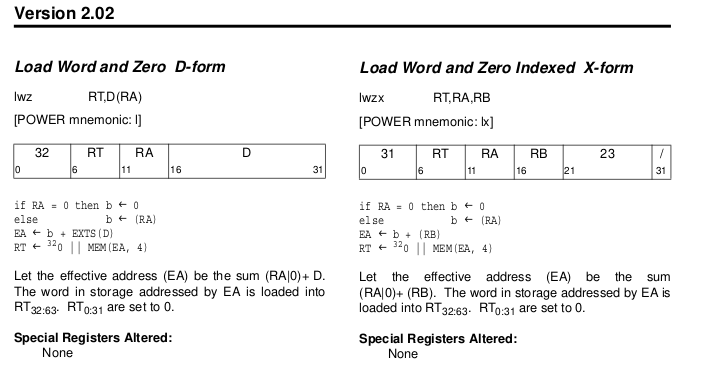
\includegraphics[width=0.9\textwidth]{powerpc-load-instr}
  

\end{frame}

\begin{frame}
  \frametitle{logiciel et architecture des microprocesseurs}
  \framesubtitle{Exemple: Architecture PowerPC : écriture d'un registre}
  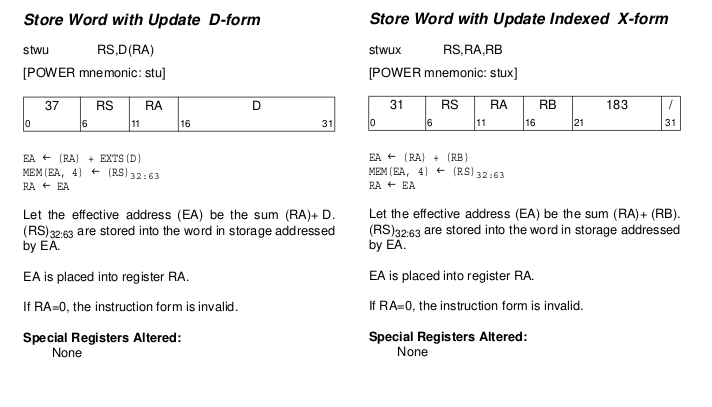
\includegraphics[width=0.9\textwidth]{powerpc-store-instr}
  

\end{frame}


\begin{frame}
  \frametitle{logiciel et architecture des microprocesseurs}
  \framesubtitle{Exemple: Architecture PowerPC : multiplication}
  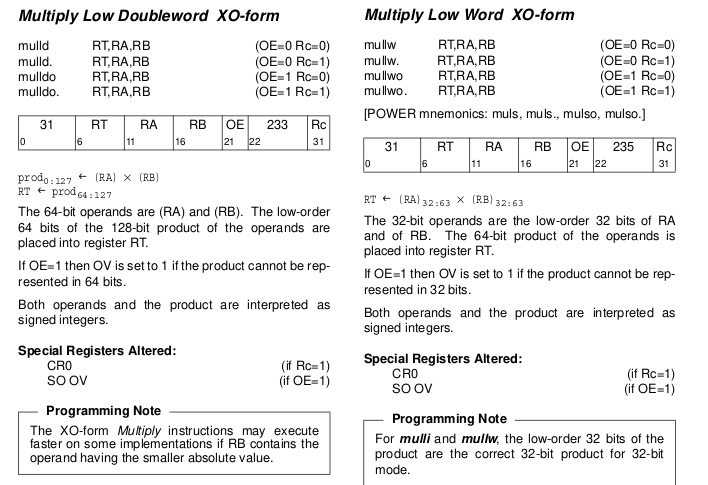
\includegraphics[width=0.9\textwidth]{powerpc-mult-instr}
\end{frame}

\begin{frame}
  \frametitle{logiciel et architecture des microprocesseurs}
  \framesubtitle{Exemple: Architecture PowerPC : comparaison}
  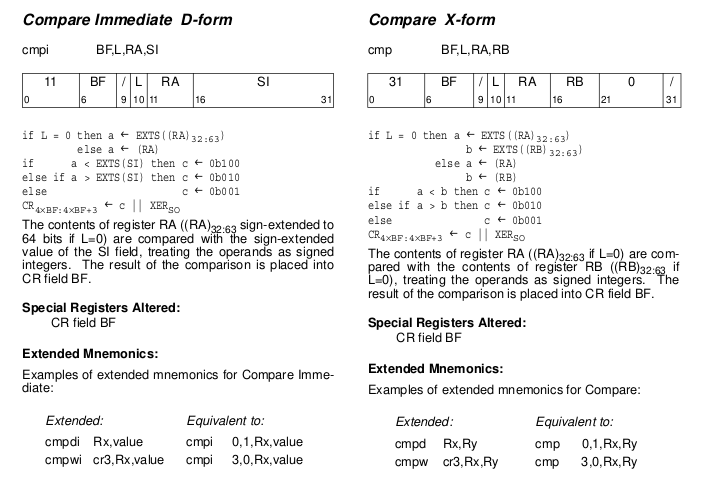
\includegraphics[width=0.9\textwidth]{powerpc-compare-instr}
\end{frame}

\begin{frame}
  \frametitle{logiciel et architecture des microprocesseurs}
  \framesubtitle{Exemple: Architecture PowerPC : branchement}
  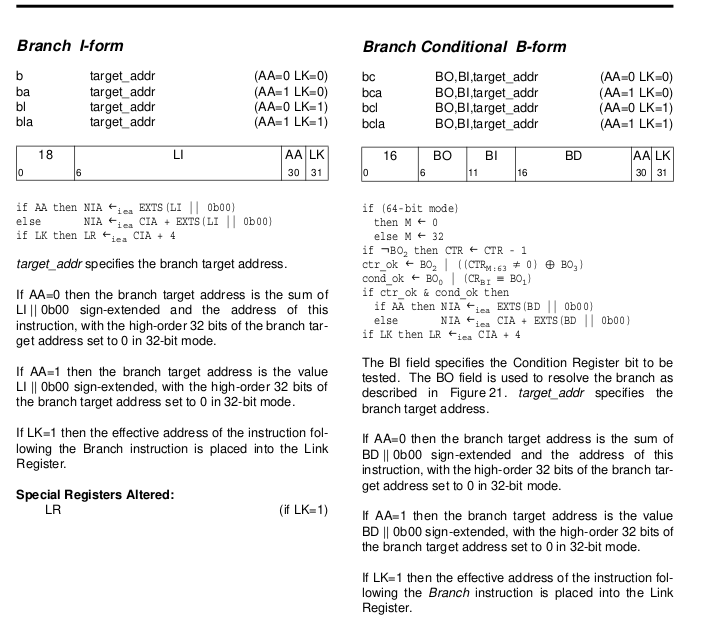
\includegraphics[width=0.7\textwidth]{powerpc-branch-instr}
\end{frame}



%%%%%%%%%%%%%%%%%%%%%%%%%%%%%%%%%%%%%%%%%%%%%%%%%%%%%%%%%%%%%%%%
\subsection{rôles et traits du noyau Linux}
\begin{frame}
  \frametitle{Le noyau Linux}
  \framesubtitle{abstraction et services fournis par le noyau Linux aux applications}

  
  \begin{itemize}

  \item Linux est \textcolor{red}{\textbf{multi-tâches}}, \textcolor{red}{\textbf{multi-utilisateurs}}

  \item les \textbf{fichiers} et \textbf{répertoires}

  \item les \textbf{processus}  {\relsize{-1}{(un programme en train de tourner)}} et les threads (filaments) - leur  \textcolor{red}{\textbf{isolation}}

  \item l'\textbf{exécution d'un fichier exécutable}

    \item la \textbf{mémoire virtuelle}
    
  \item la \textbf{communication entre processus}

  \item la \textbf{gestion des périphériques} {\relsize{-1}{(écran, clavier, souris, clef USB, disque, ....)}}

  \item le \textbf{réseau} {\relsize{-1}{(Internet)}} et la \textbf{communication entre ordinateurs} {\relsize{-1}{(Ethernet, Wifi, ....)}}

  \end{itemize}

   \textcolor{red}{\textbf{Le noyau Linux fournit les appels systèmes}} listés en \href{https://man7.org/linux/man-pages/man2/syscalls.2.html}{syscalls(2)}
\end{frame}

\begin{frame}
  \frametitle{Le noyau Linux}
  \framesubtitle{La ``philosophie d'Unix''}

  \href{https://en.wikipedia.org/wiki/Unix_philosophy}{Unix philosophy} (wikipedia)

  \begin{relsize}{-0.6}
The Unix philosophy, originated by Ken Thompson, is a set of cultural
norms and philosophical approaches to minimalist, modular software
development. It is based on the experience of leading developers of
the Unix operating system. Early Unix developers were important in
\textbf{bringing the concepts of modularity and reusability into software
engineering practice}, spawning a "software tools" movement. Over time,
the leading developers of Unix (and programs that ran on it)
established a set of cultural norms for developing software; these
norms became as important and influential as the technology of Unix
itself; this has been termed the "Unix philosophy."

The Unix philosophy emphasizes building simple, short, clear, modular,
and extensible code that can be easily maintained and repurposed by
developers other than its creators. \textbf{The Unix philosophy favors
composability as opposed to monolithic design}.
  \end{relsize}

  \vspace{0.3cm}

  \begin{relsize}{-0.5}
   \textcolor{DarkGreen}{Accepter de mal faire quand ça marche souvent, pour faciliter le travail des collègues....}
  \end{relsize}
\end{frame}


\begin{frame}
  \frametitle{Le noyau Linux}
  \framesubtitle{mémoire virtuelle}

  Les addresses (par exemple sur 32 bits) dans les registres ne correspondent pas \textbf{directement} à la mémoire physique DRAM.

  Le noyau du système d'exploitation gère la \href{https://fr.wikipedia.org/wiki/Mémoire_virtuelle}{mémoire virtuelle} (Wikipedia)

  \begin{tabular}{l|p{8.5cm}}
    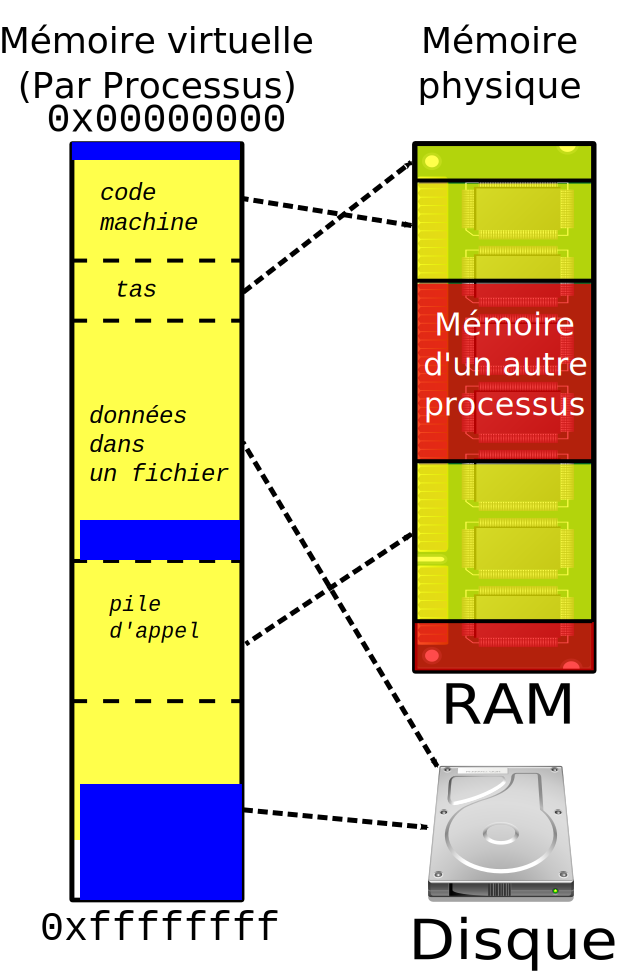
\includegraphics[width=0.30\textwidth]{Memoire-virtuelle} & %
    \begin{minipage}[b]{7cm}
      \begin{itemize}
      \item l'\textbf{espace d'adressage} d'un processus est géré par \textbf{pages} de 4Ko
      \item une page pourrait être (pour son processus): \begin{enumerate}
      \item interdite d'accès (en bleu)
      \item partagée avec d'autres processus
      \item projetée (en lecture, en écriture) sur un bout de fichier
      \item avec/sans du code machine exécutable 
      \item à lecture seule
      \item à lecture et écriture
      \end{enumerate}
      \end{itemize}
    \end{minipage}
  \end{tabular}
\end{frame}

\begin{frame}
  \frametitle{Le noyau Linux}
  \framesubtitle{pagination de la mémoire virtuelle}

  Commande Linux
  \href{https://man7.org/linux/man-pages/man1/pmap.1.html}{pmap(1)}
  utilisant le système de pseudo-fichiers \texttt{/proc/}, voir
  \href{https://man7.org/linux/man-pages/man5/proc.5.html}{proc(5)} et (pour cyber-sécurité) \href{https://fr.wikipedia.org/wiki/Address_space_layout_randomization}{Address space layout randomization}

  Essayez \texttt{pmap \$\$} puis \texttt{/bin/cat /proc/self/maps} dans un terminal de commandes

  Ou bien avec \texttt{sash}, le \href{https://en.wikipedia.org/wiki/Stand-alone_shell}{stand-alone shell}

      \begin{alltt}
    pmap 41424\\
    41424:   sash\\
    0000000000400000   1088K r-x-- sash\\
    0000000000710000     28K rw--- sash\\
    0000000000717000     12K rw---   [ anon ]\\
    000000000217e000    140K rw---   [ anon ]\\
    00007ffc09812000    132K rw---   [ pile  ]\\
    00007ffc0989b000     12K r----   [ anon ]\\
    00007ffc0989e000      4K r-x--   [ anon ]\\
    ffffffffff600000      4K --x--   [ anon ]\\
     total             1420K
      \end{alltt}
  
\end{frame}

\begin{frame}
  \frametitle{Le noyau Linux}
  \framesubtitle{systèmes de fichiers - abstraction}


  Les fichiers et répertoires ``n'existent pas'' et sont  \textbf{\textcolor{red}{une abstraction}} fournie par le noyau du système d'exploitation. \textbf{\textcolor{red}{Les fichiers sont des séquences d'octets}} {\relsize{-1}{(souvent une dizaine, parfois des milliards)}} \textbf{\textcolor{red}{avec des méta-données}}.

  Conventions de nommage et d'accès (simplifiées)

  \begin{itemize}

  \item conventions des fichiers sous Linux documentées dans \href{https://man7.org/linux/man-pages/man7/hier.7.html}{\texttt{hier(7)}} \begin{itemize}
  \item \texttt{/bin/} et \texttt{/sbin/}: executables essentiels.
  \item \texttt{/usr/bin/} et \texttt{/usr/sbin/}: executables usuels.
    \item \texttt{/etc/} : fichiers de configuration du système. Par
      exemple \texttt{/etc/passwd} décrit les utilisateurs (et parfois
      leur mot de passe), voir
      \href{https://man7.org/linux/man-pages/man5/passwd.5.html}{passwd(5)}. \texttt{/etc/X11/xorg.conf}
      configure le gestionnaire de fenêtres graphiques
      \href{https://fr.wikipedia.org/wiki/X.Org}{X.Org}.
      \item \texttt{/home/} : contient les répertoires domestiques (``home directory'') de chaque utilisateur. Par exemple \texttt{/home/basile/}
      \item \texttt{/dev/} : contient les pseudo-fichiers correspondant aux périphériques {\relsize{-1}{(``device'', par exemple \texttt{/dev/cdrom} ou \texttt{/dev/zero}  ou   \texttt{/dev/random})}}.
  \end{itemize}
    \item les \textbf{répertoires}, les  \textbf{liens symboliques} sont des fichiers.
  \end{itemize}

\end{frame}
  
\begin{frame}
  \frametitle{Le noyau Linux}
  \framesubtitle{systèmes de fichiers - conseils de nommage}

  Voir \href{https://man7.org/linux/man-pages/man7/path_resolution.7.html}{\texttt{path\_resolution(7)}} pour ``comment ça marche''
  
  \begin{itemize}
  \item \textcolor{FireBrick}{éviter les caractères bizarres}, par exemple espace, point-virgule ou tabulation
  \item \textcolor{DarkGreen}{commencer et terminer un nom de fichier par une lettre ou chiffre ou blanc-souligné {\texttt{\_}}}
  \item les fichiers dont le nom commencent par un point \texttt{.} sont ``cachés''
  \item les chemins \texttt{.} et \texttt{..} désignent le répertoire courant ou parent
    \item l'extension (après un point) désigne par convention le type de contenu: \texttt{.html} pour du web, \texttt{.pdf} pour un document PDF, \texttt{.c} pour du code C, \texttt{.s} pour du code assembleur, \texttt{.so} pour une bibliothèque partagée ou un greffon (voir \href{https://man7.org/linux/man-pages/man3/dlopen.3.html}{dlopen(3)}), \textbf{etc...}
  \end{itemize}


  \vspace{0.3cm}
  
  \textbf{\textcolor{red}{importance de suivre les conventions}}
\end{frame}


\begin{frame}
  \frametitle{Le noyau Linux}
  \framesubtitle{types de fichiers (vue statique)}

  Un \textbf{\textcolor{red}{fichier}} peut être:

  \begin{itemize}

  \item un \textbf{\textcolor{red}{fichier ordinaire}} (``plain file'') octets) - par exemple un document LibreOffice ou un executable

  \item un  \textbf{\textcolor{red}{répertoire}} (``directory'') associant des noms à des fichiers

  \item un \textbf{\textcolor{red}{lien symbolique}} \href{https://man7.org/linux/man-pages/man7/symlink.7.html}{symlink(7)}

  \item les liens durs (``hard links'') traduisent le fait qu'un même fichier peut avoir plusieurs noms
    
    \item un \textbf{\textcolor{red}{canal nommé}} \href{https://man7.org/linux/man-pages/man7/fifo.7.html}{fifo(7)}
  \end{itemize}


  \vspace{0.3cm}

  Un fichier peut ne pas avoir de nom ou en avoir plusieurs. Le plus souvent, un fichier a un nom.

  Utiliser les commandes
  \href{https://man7.org/linux/man-pages/man1/ls.1.html}{ls(1)},
  \href{https://man7.org/linux/man-pages/man1/stat.1.html}{stat(1)},
  \href{https://man7.org/linux/man-pages/man1/find.1.html}{find(1)},
  \href{https://man7.org/linux/man-pages/man1/df.1.html}{df(1)},
  \href{https://man7.org/linux/man-pages/man1/du.1.html}{du(1)} pour
  interroger un système Linux sur ses fichiers, et dans un programme
  les appels systèmes
  \href{https://man7.org/linux/man-pages/man2/stat.2.html}{stat(2)} et
  les fonctions
  \href{https://man7.org/linux/man-pages/man3/opendir.3.html}{opendir(3)},
  \href{https://man7.org/linux/man-pages/man3/readdir.3.html}{readdir(3)},
  \href{https://man7.org/linux/man-pages/man3/nftw.3.html}{nftw(3)}
  pour interroger un répertoire.
  
\end{frame}


\begin{frame}
  \frametitle{Le noyau Linux}
  \framesubtitle{systèmes de fichiers et montage} 

Un  \textbf{\textcolor{red}{système de fichiers}} (``file system'') regroupe une sous-arborescence de fichiers dans un même disque ou partition

\vspace{0.5cm}

Il existe plusieurs types de systèmes de fichiers (Ext3, Ext4, XFS, ...)
  \href{https://man7.org/linux/man-pages/man5/ext4.5.html}{ext4(5)},
  \href{https://man7.org/linux/man-pages/man5/xfs.5.html}{xfs(5)}

\vspace{0.5cm}

Il existe des systèmes de fichiers distants (NFS, CIFS)
  \href{https://man7.org/linux/man-pages/man5/nfs.5.html}{nfs(5)}

\vspace{0.5cm}

Linux sait \textbf{\textcolor{red}{monter un système de fichiers}} sur un répertoire 
\href{https://man7.org/linux/man-pages/man8/mount.8.html}{mount(8)}
  \href{https://man7.org/linux/man-pages/man5/fstab.5.html}{fstab(5)}

\vspace{0.5cm}

Sur les supercalculateurs: milliards de fichiers, système de fichiers géants (peta-octets) distribués

\end{frame}


\begin{frame}
  \frametitle{Le noyau Linux}
  \framesubtitle{contrôle et droits d'accès, propriétaires et groupes}

   \textbf{\textcolor{red}{Les fichiers comme les processus ont}} chacun :

  \begin{itemize}

  \item \textbf{\textcolor{red}{un propriétaire}} ou utilisateur (désigné par un numéro, ``owner user id'')

  \item \textbf{\textcolor{red}{un groupe}} (désigné par un numéro, ``group id'')

  \item \textbf{\textcolor{red}{des droits d'accès}} pour le propriétaire, le groupe, les autres

  \end{itemize}

  L'utilisateur 0 est spécial: \textbf{\textcolor{brown}{root}} et ``peut tout faire''

\vspace{0.5cm}

  La correspondance entre numéro d'utilisateur et son nom est décrite
  par le fichier \texttt{/etc/passwd} (voir
  \href{https://man7.org/linux/man-pages/man5/passwd.5.html}{passwd(5)})
  accessible par les fonctions
  \href{https://man7.org/linux/man-pages/man3/getpwuid.3.html}{getpwuid(3)}
  et suivantes.
  
  La correspondance entre numéro de groupe et son nom est décrite
  par le fichier \texttt{/etc/group} (voir
  \href{https://man7.org/linux/man-pages/man5/group.5.html}{group(5)})
  accessible par les fonctions
  \href{https://man7.org/linux/man-pages/man3/getgrgid.3.html}{getgrgid(3)}
  et suivantes.
  
\end{frame}

\subsection{fichiers et processus}

\begin{frame}
  \frametitle{Fichiers et processus}
  \framesubtitle{méta-données des fichiers}

  Voir \href{https://man7.org/linux/man-pages/man7/inode.7.html}{inode(7)} pour les détails, et \href{https://man7.org/linux/man-pages/man2/stat.2.html}{stat(2)} pour les interroger programmatiquement.

  \begin{relsize}{-0.5}
  \begin{itemize}
  \item taille du fichier (en octets) et taille occupée en blocs
    \item en option date de création {\relsize{-1}{(en secondes par rapport à l'\href{https://fr.wikipedia.org/wiki/Epoch}{Epoch}, début de l'année 1970)}}
    \item date de dernière modification ou changement (en secondes)
    \item date de dernier accès (en secondes ou mieux)
    \item système de fichiers et périphérique le contenant
    \item type de fichier (ordinaire, lien symbolique, FIFO, répertoire, etc...)
    \item compteur de liens (ou de noms)
    \item utilisateur propriétaire (user id) et groupe propriétaire (group id)
    \item droit d'accès (\texttt{rwx}) lecture, écriture, exécution pour l'utilisateur
    \item droit d'accès (\texttt{rwx}) lecture, écriture, exécution pour le groupe
    \item droit d'accès (\texttt{rwx}) lecture, écriture, exécution pour les autres
  \end{itemize}
  \end{relsize}
\end{frame}

\begin{frame}
  \frametitle{Fichiers et processus}
  \framesubtitle{exemple de méta-données d'un fichier}
  
        Exemple avec la commande
        \href{https://man7.org/linux/man-pages/man2/stat.1.html}{stat(1)}
        utilisant
        \href{https://man7.org/linux/man-pages/man2/stat.2.html}{stat(2)}
        : \\ \texttt{stat intro-programmation-sous-Linux.tex} produit
        :

        \begin{relsize}{-0.5}
        \begin{alltt}
          Fichier : intro-programmation-sous-Linux.tex\\
         Taille : 33520     	Blocs : 72         Blocs d'E/S : 4096   fichier \\
      Périphérique: 802h/2050d	Inœud: 918078      Liens: 1\\
      Accès: (0644/-rw-r--r--)  UID: (12752/basilest)   GID: ( 4200/basilegr)\\
      Accès: 2020-08-02 12:40:26.275083457 +0200\\
      Modif.: 2020-08-02 12:40:20.153093527 +0200\\
      Changt: 2020-08-02 12:40:20.153093527 +0200\\
        Créé: -
        \end{alltt}
        \end{relsize}
\end{frame}

\begin{frame}
  \frametitle{Fichiers et processus}
  \framesubtitle{les fichiers exécutables}

  Le noyau Linux peut exécuter dans un processus avec l'appel système
  \href{https://man7.org/linux/man-pages/man2/execve.2.html}{execve(2)} {\relsize{-1}{(re-initialisant l'espace d'adressage et les registres de ce processus)}} :

  \begin{itemize}

  \item un fichier de script {\relsize{-1}{(lisible et executable, débutant par
      le \href{https://fr.wikipedia.org/wiki/Shebang}{shebang}
    {\textcolor{brown}{\textbf{\texttt{\#!}}}}
      )}}

    \item un exécutable binaire au format 
      \href{https://man7.org/linux/man-pages/man5/elf.5.html}{elf(5)} {\relsize{-1}{(voir wikipage \href{https://fr.wikipedia.org/wiki/Executable_and_Linkable_Format}{Executable and Linkable Format})}}
      avec des ``octets magiques'' (\textit{magic number}): \\
      
  \begin{tabular}{l|p{7.5cm}}
    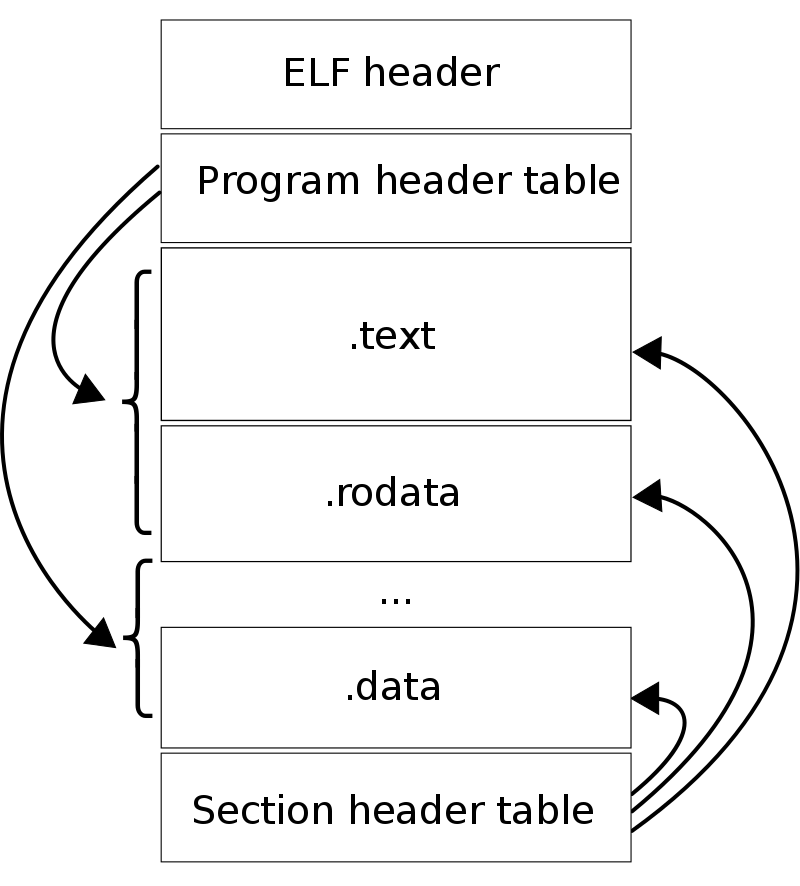
\includegraphics[width=0.3\textwidth]{Elf-layout} &
    \begin{relsize}{-1}
  \begin{minipage}[b]{6.5cm}
    Similitude voulue avec l'espace d'adressage :
    \begin{itemize}
    \item \textit{certaines sections} correspondent à des \textit{segments} de l'espace d'adressage
    \item d'autres sections ne sont pas projetées dans la mémoire virtuelle. \\ Par exemple: \textit{informations de déboguage} au format \href{https://en.wikipedia.org/wiki/DWARF}{DWARF} ou \href{https://fr.wikipedia.org/wiki/Table_des_symboles}{table des symboles}.
    \end{itemize}
  \end{minipage}
    \end{relsize}
  \end{tabular}
  \end{itemize}
\end{frame}


\begin{frame}
  \frametitle{Fichiers et processus}
  \framesubtitle{Analyser ou modifier le contenu d'un fichier}
  
  De nombreuses commandes existent. On peut en créer d'autres...
  \begin{itemize}
    
    \item dump en octal  \href{https://man7.org/linux/man-pages/man1/od.1.html}{od(1)} ou en hexadécimal \href{https://man7.org/linux/man-pages/man1/hd.1.html}{hd(1)} 

    \item lignes de tête \href{https://man7.org/linux/man-pages/man1/head.1.html}{head(1)}  ou de queue \href{https://man7.org/linux/man-pages/man1/tail.1.html}{tail(1)} 

    \item concatener plusieurs fichiers \href{https://man7.org/linux/man-pages/man1/cat.1.html}{cat(1)}
    \item recherche  \href{https://man7.org/linux/man-pages/man1/grep.1.html}{grep(1)}
    \item édition par flots  \href{https://man7.org/linux/man-pages/man1/sed.1.html}{sed(1)}
      
    \item copie \href{https://man7.org/linux/man-pages/man1/cp.1.html}{cp(1)} , suppression \href{https://man7.org/linux/man-pages/man1/rm.1.html}{rm(1)}, renommage \href{https://man7.org/linux/man-pages/man1/mv.1.html}{mv(1)}

    \item sur un fichier exécutable \href{https://fr.wikipedia.org/wiki/Executable_and_Linkable_Format}{ELF} :

      \begin{itemize}
      \item commande  \href{https://man7.org/linux/man-pages/man1/nm.1.html}{nm(1)} pour la table des noms (symboles)

        \item  commande  \href{https://man7.org/linux/man-pages/man1/readelf.1.html}{readelf(1)} pour extraire des informations
        \item  commande  \href{https://man7.org/linux/man-pages/man1/objdump.1.html}{objdump(1)} pour afficher des informations
        \item  commande  \href{https://man7.org/linux/man-pages/man1/ldd.1.html}{ldd(1)} pour lister les dépendances
      \end{itemize}
  \end{itemize}
\end{frame}
      

\begin{frame}
  \frametitle{Fichiers et processus}
  \framesubtitle{Les processus}

     \textbf{\textcolor{red}{Chaque processus est un programme \textcolor{FireBrick}{-fichier exécutable-} en train de tourner}} -en cours
  d'exécution-.  {\relsize{-1}{Méta-données descriptives décrites dans
  \href{https://man7.org/linux/man-pages/man7/credentials.7.html}{credentials(7)}
  et accessibles via
  \href{https://man7.org/linux/man-pages/man5/proc.5.html}{proc(5)},
  notamment \texttt{/proc/self/} pour le processus courant}}

  \begin{relsize}{-0.5}
  \begin{itemize}

  \item commandes
    \href{https://man7.org/linux/man-pages/man1/ps.1.html}{ps(1)},
    \href{https://man7.org/linux/man-pages/man1/pstree.1.html}{pstree(1)}
    et \href{https://man7.org/linux/man-pages/man1/top.1.html}{top(1)}
    pour les lister {\relsize{-1}{(via le pseudo-système de fichiers
        \texttt{/proc/})}}
    
  \item un même exécutable (ou script) peut être exécuté par \emph{plusieurs}
    processus en parallèle {\relsize{-1}{(exécution concurrente, en particulier
    l'interprète de commande
    \href{https://man7.org/linux/man-pages/man1/bash.1.html}{bash(1)}
    qui lance des processus à partir de commandes)}}

  \item \textbf{chaque processus a son propre espace d'adressage} virtuel modifiable par
  \href{https://man7.org/linux/man-pages/man2/execve.2.html}{execve(2)},
  \href{https://man7.org/linux/man-pages/man2/mmap.2.html}{mmap(2)},
  \href{https://man7.org/linux/man-pages/man2/munmap.2.html}{munmap(2)},
  \href{https://man7.org/linux/man-pages/man2/sbrk.2.html}{sbrk(2)},
  \href{https://man7.org/linux/man-pages/man2/mprotect.2.html}{mprotect(2)}

    \item  \textbf{chaque processus a son identifiant unique numérique} (pid, ``process id'')
 accessible par \href{https://man7.org/linux/man-pages/man2/getpid.2.html}{getpid(2)}
    
    \item \textbf{chaque processus est créé par son processus père} {\relsize{-1}{(sauf \texttt{/sbin/init}, de pid 1, démarré automagiquement par le noyau)}} dont le pid est renvoyé par
  \href{https://man7.org/linux/man-pages/man2/getppid.2.html}{getppid(2)}. Il peut survivre à son père.
    
  \end{itemize}
  \end{relsize}
  
\end{frame}

\begin{frame}
  \frametitle{Fichiers et processus}
  \framesubtitle{création et terminaison des processus}

  \textbf{\textcolor{red}{Création d'un processus:}} par \textbf{l'appel
  système
  \href{https://man7.org/linux/man-pages/man2/fork.2.html}{fork(2)}},
  qui peut échouer, et quand il réussit créer par ``clonage'' un processus fils quasi
  identique au père, et \textbf{a \textcolor{FireBrick}{deux résultats}} : 0 dans le fils, et le pid
  du fils dans le père.

  \vspace{0.5cm}
  \textbf{\textcolor{red}{Terminaison d'un processus:}}

  \begin{itemize}
    \item \textbf{\textcolor{FireBrick}{terminaison normale}} explicite par
      \href{https://man7.org/linux/man-pages/man2/exit.2.html}{\texttt{\_exit(2)}} ou
      \href{https://man7.org/linux/man-pages/man3/exit.3.html}{\texttt{exit(3)}} ou \textbf{fin normale du programme}

    \item \textbf{\textcolor{FireBrick}{terminaison prématurée}} en
      erreur par un signal (voir
      \href{https://man7.org/linux/man-pages/man7/signal.7.html}{signal(7)})
      forcé par \textbf{un plantage} (ou abus de resources; cf \href{https://man7.org/linux/man-pages/man2/setrlimit.2.html}{setrlimit(2)}) du
      programme de ce processus {\relsize{-1}{(division par 0, viol de
          l'espace d'adressage, dépassement de temps alloué,
          débordement d'espace disque, ...)}}
      
    \item \textbf{\textcolor{FireBrick}{terminaison forcée}} par un signal (voir 
  \href{https://man7.org/linux/man-pages/man7/signal.7.html}{signal(7)}) \textbf{émis par un processus tueur} via 
     l'appel système \href{https://man7.org/linux/man-pages/man2/kill.2.html}{\texttt{kill(2)}} ou la commande \href{https://man7.org/linux/man-pages/man1/kill.1.html}{\texttt{kill(1)}}. Les droits d'accès s'appliquent.
  \end{itemize}
  
\end{frame}
\begin{frame}
  \frametitle{Fichiers et processus}
  \framesubtitle{attente et observation dynamique d'un processus}

  \textbf{\textcolor{red}{Attente d'un processus}}: l'appel système
  \href{https://man7.org/linux/man-pages/man2/wait.2.html}{\texttt{wait(2)}}
  attend un fils quelconque. Et
  \href{https://man7.org/linux/man-pages/man2/waitpid.2.html}{\texttt{waitpid(2)}}
  attend un fils donné (ou un groupe de fils). Un shell comme \href{https://man7.org/linux/man-pages/man1/bash.1.html}{\texttt{bash(1)}} lance et attend plein de fils (un par commande lancée).


  \vspace{0.4cm}
  
  Plusieurs manières d'\textbf{\textcolor{red}{observer un processus}} donné:

  \begin{itemize}

  \item l'appel système de bas niveau \href{https://man7.org/linux/man-pages/man2/ptrace.2.html}{\texttt{ptrace(2)}}
 
    
  \item la commande
    \href{https://man7.org/linux/man-pages/man1/strace.1.html}{\texttt{strace(1)}}
    liste les appels systèmes, et
    \href{https://man7.org/linux/man-pages/man1/ltrace.1.html}{\texttt{ltrace(1)}}
    liste les appels de fonctions de bibliothèque.

    \item le débogueur 
    \href{https://man7.org/linux/man-pages/man1/gdb.1.html}{\texttt{gdb(1)}} profite des informations de déboguage
    
    \item le chronomètre 
    \href{https://man7.org/linux/man-pages/man1/time.1.html}{\texttt{time(1)}} mesure les temps passés  (voir 
  \href{https://man7.org/linux/man-pages/man7/time.7.html}{time(7)} pour les détails)
    
    \item l'utilitaire 
    \href{https://man7.org/linux/man-pages/man1/perf.1.html}{\texttt{perf(1)}} analyse les performances
    
  \end{itemize}
  
\end{frame}

\begin{frame}
  \frametitle{Fichiers et processus}
  \framesubtitle{table de descripteurs de fichiers}

  \textbf{Chaque processus Linux a sa propre}
  \textbf{\textcolor{red}{table de descripteurs de fichiers}} ouverts
    (``open file descriptor table'', moins d'une dizaine à des
    milliers d'entrées), voir
    \href{https://man7.org/linux/man-pages/man3/stdio.3.html}{stdio(3)}. Conventionnellement
    souvent au moins:

  \begin{itemize}
    \item[\texttt{0}]  \textbf{entrée standard} \texttt{STDIN\_FILENO}, en C le canal \texttt{stdin}
    \item[\texttt{1}]   \textbf{sortie standard} \texttt{STDOUT\_FILENO}, en C le canal \texttt{stdout}
    \item[\texttt{2}]   \textbf{message d'erreurs standard} \texttt{STDERR\_FILENO}, en C le canal \texttt{stderr}
  \end{itemize}

  \vspace{0.3cm}

  Certains processus Linux (notamment les logiciels serveurs Web)
  peuvent avoir des dizaines de milliers de descripteurs de fichiers
  (une par connection TCP/IP). On peut en limiter le nombre par
  \href{https://man7.org/linux/man-pages/man2/setrlimit.2.html}{setrlimit(2)}
  et ces limites sont héritées par le processus fils créé par
  \href{https://man7.org/linux/man-pages/man2/fork.2.html}{fork(2)}. Utiliser
  \texttt{/proc/self/fd/} pour consulter cette table comme un
  pseudo-répertoire.
\end{frame}

\begin{frame}
  \frametitle{Fichiers et processus}
  \framesubtitle{modification de la table de descripteurs de fichiers}


  
  Les appels systèmes suivants modifient cette table (copiée par
  \href{https://man7.org/linux/man-pages/man2/fork.2.html}{fork(2)}) :

  \begin{itemize}
    \item 
  \href{https://man7.org/linux/man-pages/man2/open.2.html}{open(2)} pour \textbf{ouvrir un fichier} existant, donné par son chemin (absolu, par exemple \texttt{/etc/fstab} ou relatif comme \texttt{../rps\_manifest.json} ou \texttt{doc/garbage-collection.md}) et 
  \href{https://man7.org/linux/man-pages/man2/creat.2.html}{creat(2)} pour  \textbf{créer un nouveau fichier}

  \item 
  \href{https://man7.org/linux/man-pages/man2/close.2.html}{close(2)} pour  \textbf{fermer un descripteur de fichiers}

\item
  \href{https://man7.org/linux/man-pages/man2/dup2.2.html}{dup2(2)}
  pour  \textbf{dupliquer un descripteur} de fichiers

\item 
  \href{https://man7.org/linux/man-pages/man2/pipe.2.html}{pipe(2)}
  pour  \textbf{créer les deux bouts d'un tube de communication} (cf
  \href{https://man7.org/linux/man-pages/man7/pipe.7.html}{pipe(7)})
  
    \item 
  \href{https://man7.org/linux/man-pages/man2/socket.2.html}{socket(2)},
  \href{https://man7.org/linux/man-pages/man2/accept.2.html}{accept(2)},
  \href{https://man7.org/linux/man-pages/man2/accept.2.html}{connect(2)} pour  \textbf{les connections réseau} (par exemple en
  \href{https://man7.org/linux/man-pages/man7/tcp.7.html}{tcp(7)})
    \item \textbf{\textcolor{red}{etc...}}
  \end{itemize}

    
\end{frame}
%%%%%%%%%%%%%%%%%%%%%%%%%%%%%%%%%%%%%%%%%%%%%%%%%%%%%%%%%%%%%%%%
%%%%%%%%%%%%%%%%%%%%%%%%%%%%%%%%%%%%%%%%%%%%%%%%%%%%%%%%%%%%%%%%

\begin{frame}
  {\Large deuxième jour}

  \vspace{0.5cm}
  \textcolor{red}{\Large *********************}
  
  \vspace{0.5cm}
  
   \tableofcontents
\end{frame}

%%================================================================
%%================================================================


\begin{frame}
  \frametitle{Fichiers et processus}
  \framesubtitle{contexte d'exécution d'un processus: répertoire courant, etc...}

  Voir
  \href{https://man7.org/linux/man-pages/man7/credentials.7.html}{credentials(7)},
  \href{https://man7.org/linux/man-pages/man7/namespaces.7.html}{namespaces(7)},
  \href{https://man7.org/linux/man-pages/man7/capabilities.7.html}{capabilities(7)}
  \href{https://man7.org/linux/man-pages/man7/pid\_namespaces.7.html}{pid\_namespaces(7)}

   \textbf{\textcolor{red}{Chaque processus a}} (cf  \href{https://man7.org/linux/man-pages/man2/fork.2.html}{fork(2)}):

  \begin{itemize}
  \item  \textbf{\textcolor{red}{son répertoire courant}} (current working directory)  (cf  \href{https://man7.org/linux/man-pages/man2/getcwd.2.html}{getcwd(2)} et \href{https://man7.org/linux/man-pages/man2/chdir.2.html}{chdir(2)} pour le changer)

  \item  \textbf{\textcolor{red}{son espace d'adressage}} dont la pile d'appel et l'environnement
    
  \item  \textbf{\textcolor{red}{sa table de descripteur de fichiers}}

    \item  \textbf{\textcolor{red}{etc...}} (par exemple, traitement des signaux, limites de resources, son répertoire racine \href{https://man7.org/linux/man-pages/man2/chroot.2.html}{chroot(2)})
    
  \end{itemize}
  
\end{frame}

\begin{frame}
  \frametitle{Fichiers et processus}
  \framesubtitle{démarrage d'un programme dans un processus par \texttt{execve}}

   \textbf{\textcolor{red}{le \textit{seul} moyen de démarrer un programme}}
   Linux, c'est l'appel système
   \href{https://man7.org/linux/man-pages/man2/execve.2.html}{\textbf{execve(2)}}
   qui ``initialise'' le processus courant pour un nouveau programme,
   ou les fonctions qui l'utilisent:
   \href{https://man7.org/linux/man-pages/man3/exec.3.html}{exec(3)}

   Cet 
   \href{https://man7.org/linux/man-pages/man2/execve.2.html}{execve(2)} prend comme arguments:

   \begin{itemize}
   \item le chemin du fichier exécutable {\relsize{-1}{(ELF ou script)}} à exécuter  \fbox{\textcolor{FireBrick}{\texttt{/bin/ls}}}

   \item le tableau des arguments (chaînes de caractères comme
     \fbox{\textcolor{FireBrick}{\texttt{ls}}}
      \fbox{\textcolor{FireBrick}{\texttt{-l}}}
      \fbox{\textcolor{FireBrick}{\texttt{mon-fichier.c}}} par exemple)
     
   \item l'environnement (tableau de chaînes de caractères comme
     \fbox{\textcolor{FireBrick}{\texttt{HOME=/home/basile}}} 
      \fbox{\textcolor{FireBrick}{\texttt{PATH=.:/bin:/usr/bin}}}...)
     
   \end{itemize}

   \begin{relsize}{-1}
   Le tableau d'arguments est connu du \texttt{main} du nouveau programme
   exécuté. L'environnement aussi (voir
   \href{https://man7.org/linux/man-pages/man7/environ.7.html}{environ(7)}
   et
   \href{https://man7.org/linux/man-pages/man3/getenv.3.html}{getenv(3)}, etc...). Les arguments et les environnements sont dans la pile d'appel du nouvel espace d'addressage.
   \end{relsize}

   Donc  \textbf{\href{https://man7.org/linux/man-pages/man2/execve.2.html}{execve(2)} est coûteux} (milliseconde parfois).
   
\end{frame}

\begin{frame}
  \frametitle{Fichiers et processus}
  \framesubtitle{mon environnement comme exemple}

La commande \href{https://man7.org/linux/man-pages/man1/printenv.1.html}{printenv(1)} me donne \relsize{-1}{(extrait \textit{incomplet}...)} :

\begin{relsize}{-1.8}
  \begin{alltt}
   SSH\_AUTH\_SOCK=/tmp/ssh-AokrAslPJO7B/agent.3033\\
   USER=basilest\\
   HOME=/home/basilest\\
   PWD=/home/basilest/introprog-montpellibre-2020\\
   LANGUAGE=fr\_FR:en\\
   LANG=fr\_FR.UTF-8\\
   LC\_IDENTIFICATION=fr\_FR.UTF-8\\
   COLORTERM=truecolor\\
  TERM=xterm-256color\\
  LC\_NUMERIC=fr\_FR.UTF-8\\
  LC\_MEASUREMENT=fr\_FR.UTF-8\\
  LC\_TIME=fr\_FR.UTF-8\\
  LC\_PAPER=fr\_FR.UTF-8\\
  PATH=/usr/local/sbin:/usr/local/bin:/usr/sbin:/usr/bin:/sbin:/bin:/snap/bin\\
  LC\_MONETARY=fr\_FR.UTF-8\\
  SHELL=/bin/zsh\\
  LC\_TELEPHONE=fr\_FR.UTF-8\\
  XAUTHORITY=/home/basilest/.Xauthority\\
  LC\_NAME=fr\_FR.UTF-8\\
  DISPLAY=:0.0\\
  LC\_ADDRESS=fr\_FR.UTF-8\\
  PS1=\%m \%3\~ ~ \%T \%\# 
  \end{alltt}
\end{relsize}
\end{frame}


\begin{frame}
  \frametitle{Fichiers et processus}
  \framesubtitle{contexte d'exécution d'un processus: conventions}
  
  @@@@ stdin, stdout, stderr, environ(7), \texttt{\$HOME} et \texttt{\$PATH}
\end{frame}


\begin{frame}
  \frametitle{Fichiers et processus}
  \framesubtitle{conventions et importance de la ligne de commande}

  @@@@
\end{frame}


\begin{frame}
  \frametitle{Fichiers et processus}
  \framesubtitle{pour en savoir plus}

  @@@@ syscalls(2), ALP, OSTEP
\end{frame}


 %%++++++++++++++++++++++++++++++++++++++++++++++++++++++++++++++++++++++
\section{Outils et langages des développeurs Linux}

\begin{frame}
  \frametitle{Outils des développeurs Linux}

  \begin{relsize}{-1}
  \begin{itemize}

  \item  \textbf{\textcolor{red}{éditeur de code source}} comme \href{https://www.gnu.org/software/emacs/}{GNU \texttt{emacs}},
    \href{https://vim.org/}{\texttt{vim}}, \href{https://help.gnome.org/users/gedit/}{\texttt{gedit}} pour créer et modifier les fichiers de code sources


  \item  \textbf{\textcolor{red}{logiciel de gestion de versions}} comme \href{https://fr.wikipedia.org/wiki/Git}{\texttt{git}} pour gérer efficacement différentes versions d'un code source
\
\item  \textbf{\textcolor{red}{forges logicielles}} par exemple  \href{https://framagit.org/}{\texttt{framagit}}

  \item  \textbf{\textcolor{red}{générateurs de code}} comme
    \href{https://fr.wikipedia.org/wiki/GNU\_Bison}{GNU
      \texttt{bison}} (génération
    d'\href{https://fr.wikipedia.org/wiki/Analyse_syntaxique}{analyse
      syntaxique}) ou \href{https://fr.wikipedia.org/wiki/SWIG}{SWIG}
    (génération de code glue)
   
  \item  \textbf{\textcolor{red}{moteur de production}} par exemple \href{https://fr.wikipedia.org/wiki/Make}{GNU \texttt{make}} ou \href{https://ninja-build.org}{\texttt{ninja}} coordonnant des outils plus élémentaires.
  \item \textbf{\textcolor{red}{interpréteurs}} (exécutant du code
    source) comme
    \href{https://man7.org/linux/man-pages/man1/bash.1.html}{\texttt{bash(1)}}
    ou \href{https://fr.wikipedia.org/wiki/Awk}{awk} ou
    \href{https://fr.wikipedia.org/wiki/GNU_Guile}{GNU Guile}
  \item  \textbf{\textcolor{red}{compilateurs}} (transformant du code source) comme \href{http://gcc.gnu.org/}{GCC} ou \href{http://ocaml.org/}{Ocaml}
  \item \textbf{\textcolor{red}{formatteurs de documents}} comme
    \href{https://fr.wikipedia.org/wiki/LaTeX}{\LaTeX} ou
    \href{https://fr.wikipedia.org/wiki/Lout}{Lout} et  \textbf{\textcolor{red}{générateurs de documentation}}
    comme \href{https://fr.wikipedia.org/wiki/Doxygen}{Doxygen}


    
    \item \href{https://fr.wikipedia.org/wiki/Programme_assembleur}{assembleurs} et \href{https://fr.wikipedia.org/wiki/Édition_de_liens}{éditeurs de liens} notamment \href{https://fr.wikipedia.org/wiki/GNU\_Binutils}{GNU \texttt{binutils}} 
    
    \item  \textbf{\textcolor{red}{bibliothèques logicielles}} comme \href{https://qt.io}{Qt} ou \href{https://fr.wikipedia.org/wiki/Ncurses}{Ncurses} etc...
      
    \item  \textbf{\textcolor{red}{débogueur}} comme 
    \href{https://man7.org/linux/man-pages/man1/gdb.1.html}{\texttt{gdb(1)}} ou \href{https://fr.wikipedia.org/wiki/Valgrind}{Valgrind}
      
  \end{itemize}
  \end{relsize}
\end{frame}

\begin{frame}
  \frametitle{Outils des développeurs Linux}
  \framesubtitle{\texttt{emacs} sur du code source C++ de \href{http://refpersys.org/}{\texttt{refpersys.org}}}

  \vspace{0.1cm}
  
    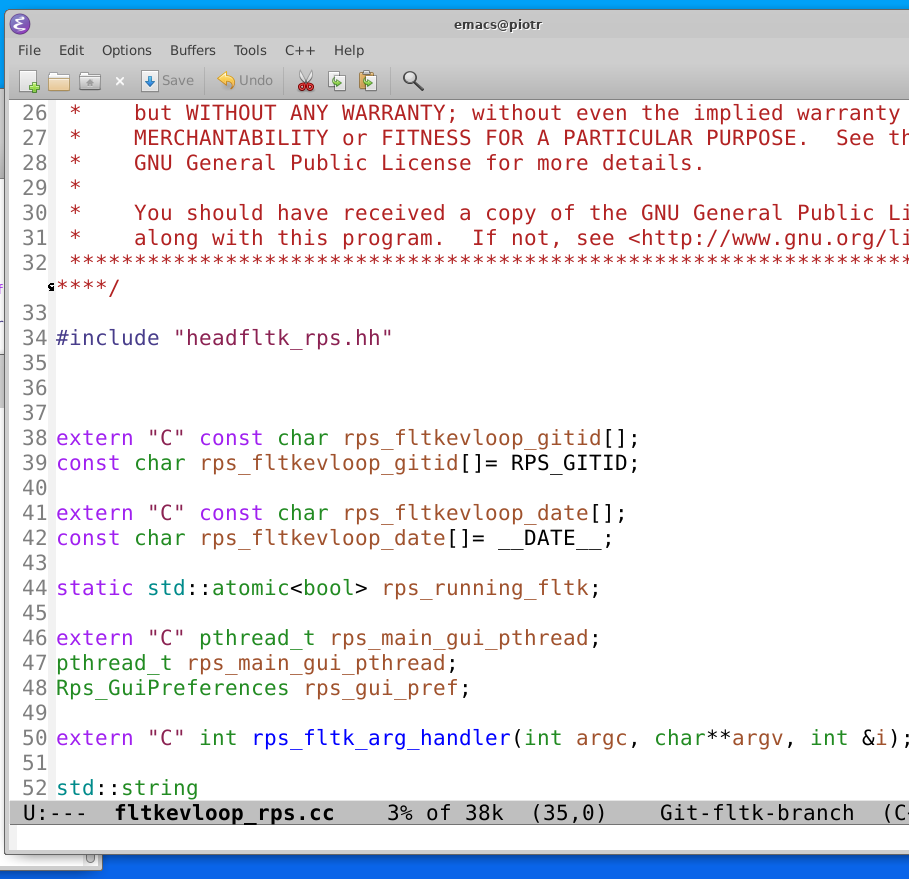
\includegraphics[width=0.66\textwidth]{emacs-refpersys} 
\end{frame}

%%%%%%%%%%%%%%%%%%%%%%%%%%%%%%%%%%%%%%%%%%%%%%%%%%%%%%%%%%%%%%%%
\begin{frame}
  \frametitle{Langages des développeurs Linux}
  \framesubtitle{problème posé}

  Exemples: compter le nombre de mots dans plusieurs fichiers, et de plus en calculer la fréquencexs
\end{frame}

\end{document}
%%%%%%%%%%%%%%%%%%%%%%%%%%%%%%%%%%%a%%%%%%%%%%%%%%%%%%%%%%%%%%
%% Local Variables: ;;
%% compile-command: "./build.sh" ;;
%% End: ;;
%%%%%%%%%%%%%%%%%%%%%%%%%%%%%%%%%%%%%%%%%%%%%%%%%%%%%%%%%%%%%%%
